\documentclass[letterpaper]{article}
\usepackage{adjustbox}
% DO NOT CHANGE THIS
\usepackage[submission]{aaai24} % DO NOT CHANGE THIS
\usepackage{times} % DO NOT CHANGE THIS
\usepackage{helvet} % DO NOT CHANGE THIS
\usepackage{courier} % DO NOT CHANGE THIS
\usepackage[hyphens]{url} % DO NOT CHANGE THIS
\usepackage{graphicx} % DO NOT CHANGE THIS
\urlstyle{rm} % DO NOT CHANGE THIS
\def\UrlFont{\rm} % DO NOT CHANGE THIS
\usepackage{natbib} % DO NOT CHANGE THIS AND DO NOT ADD ANY OPTIONS TO IT
\usepackage{caption} % DO NOT CHANGE THIS AND DO NOT ADD ANY OPTIONS TO IT
\usepackage{subcaption}
\frenchspacing % DO NOT CHANGE THIS
\setlength{\pdfpagewidth}{8.5in} % DO NOT CHANGE THIS
\setlength{\pdfpageheight}{11in} % DO NOT CHANGE THIS

\usepackage{algorithm}
\usepackage{algpseudocode}
\usepackage{caption}

\usepackage{color}
\newcommand{\omer}[1]{\textcolor{red}{\textbf{Omer Says:} #1 }}
\newcommand{\oshri}[1]{\textcolor{blue}{\textbf{Oshri Says:} #1 }}

\usepackage{amsmath,amsthm,amsfonts}
\newtheorem{observation}{Observation}
\usepackage{nicefrac}

\algrenewcommand\algorithmicrequire{\textbf{Input:}}
\algrenewcommand\algorithmicensure{\textbf{Output:}}

\usepackage{newfloat}
\usepackage{listings}
\DeclareCaptionStyle{ruled}{labelfont=normalfont,labelsep=colon,strut=off} % DO NOT CHANGE THIS
\lstset{%
basicstyle={\footnotesize\ttfamily},% footnotesize acceptable for monospace
numbers=left,numberstyle=\footnotesize,xleftmargin=2em,% show line numbers, remove this entire line if you don't want the numbers.
aboveskip=0pt,belowskip=0pt,%
showstringspaces=false,tabsize=2,breaklines=true}
\floatstyle{ruled}
\newfloat{listing}{tb}{lst}{}
\floatname{listing}{Listing}


\setcounter{secnumdepth}{0} %May be changed to 1 or 2 if section numbers are desired.



\title{Partition with Two-Stages: What Works and How?}
\author{
Written by AAAI Press Staff\textsuperscript{\rm 1}\thanks{With help from the AAAI Publications Committee.}\\
AAAI Style Contributions by Pater Patel Schneider,
Sunil Issar,\\
J. Scott Penberthy,
George Ferguson,
Hans Guesgen,
Francisco Cruz\equalcontrib,
Marc Pujol-Gonzalez\equalcontrib
}
\affiliations{
\textsuperscript{\rm 1}Association for the Advancement of Artificial Intelligence\\


1900 Embarcadero Road, Suite 101\\
Palo Alto, California 94303-3310 USA\\
proceedings-questions@aaai.org
}

\iffalse
\title{My Publication Title -- Single Author}
\author {
Author Name
}
\affiliations{
Affiliation\\
Affiliation Line 2\\
name@example.com
}
\fi

\iffalse
\title{My Publication Title -- Multiple Authors}
\author {
First Author Name\textsuperscript{\rm 1},
Second Author Name\textsuperscript{\rm 2},
Third Author Name\textsuperscript{\rm 1}
}
\affiliations {
\textsuperscript{\rm 1}Affiliation 1\\
\textsuperscript{\rm 2}Affiliation 2\\
firstAuthor@affiliation1.com, secondAuthor@affilation2.com, thirdAuthor@affiliation1.com
}
\fi



\begin{document}

\maketitle

\begin{abstract}
Peer-evaluation systems are used when sets of agents evaluate each other in order to select the best $k$ among them. These are commonly used in various real-world settings, such as in academic conferences, in which those submitting papers are also reviewing papers. Recently, conferences have attempted to focus their review resources by moving to a two-stage mechanism, in which some papers are eliminated after a first stage, and then more reviews are added to those which are left.

A major strategyproof mechanism that has been suggested for peer-evaluation is \emph{Partition}, and we investigate how this mechanism performs when adapted to a two-stage system. Unlike what may be expected, we show that the two-stage mechanism's advantage is not for papers on the threshold of acceptance, but for those below the top-most papers, but not edge-case, ranking wise. We examine how the two-stage mechanism affects the quality of the selected agents, and what are the parameters that improve its performance -- how many candidates to eliminate in the first stage, and how to divide the number of reviews between the stages. This is highly dependent on the number of required agents, the number of reviews requested from agents, and reviewers' correlation.
\end{abstract}

\section{Introduction}
Peer-evaluation, the process in which a group judges its members and selects the best, is a process humans have engaged with for thousands of years. In many ancient cases, selection by lot was done (sortition of sorts), as it was assumed there is a divine intervention (see Samuel I, chapter 10). Later, people tried to choose the best person for a job by various selection methods (e.g., the selection of the Pope from -- and by -- the College of Cardinals). While in small groups this can be akin to voting, the main difference from elections is that the set of candidates and voters are the same, and furthermore, the case of the selection of a single winner is less common in comparison to the desire to select a set of $k$ best agents (or to find a ranking of all agents).

More recently, peer-evaluation is commonly practiced in many companies and organizations, for example, as part of employees' evaluation process or advancement protocol.%\footnote{For example, it is a required part of the Israeli Army's officer training course, as well as part of its officer evaluation process.}
Academics are intimately familiar with peer evaluation, as refereed academic conferences (such as most computer-science conferences, e.g., AAAI) implement such a system: those submitting papers are often tasked with evaluating other papers. Indeed, in the past few years many conferences have decreed that paper authors must be willing to review other papers.

Research in this field has mostly focused on \emph{strategyproof} mechanisms, i.e., ways in which agents cannot improve their chances of being selected by giving an untruthful report on others. One of the initial mechanisms suggested for this was \emph{Partition}~\cite{AFPT11}, in which agents are divided into two groups, and each agent reviews agents which are not in their own group. These reviews ultimately create a ranking of each group, and the top $\frac{k}{2}$ is selected from each.

In parallel to these efforts, academic conferences have struggled to deal with a different, orthogonal problem: the problem of using a limited resource -- the number of papers that can be reviewed by agents -- with the desire to select the best set of papers. As research has shown~\cite{Law22}, reviewers are quite ``noisy'', i.e., not in agreement with each other on a ground-truth of the ranking of all papers. Therefore there is a desire to have more reviews for each paper, so as to increase the chance of getting a better signal regarding its quality. One approach to deal with this issue, initially used at the AAAI 2021 conference, and since then more widely in AI conferences, is two-stage reviewing \cite{LMNZCNR22}. In the first stage, each reviewer reviews only a few papers, and based on this relatively-noisy signal, papers which received very bad reviews are eliminated, leaving fewer papers, which reviewers' remaining reviews can be focused on. Thus, instead of all papers receiving the same amount of reviews, those eliminated in the first stage receive fewer, while the remaining ones get more, allowing, hopefully, for a better selection of the best papers.

In this paper we provide an analysis the Partition mechanism (which remains strategyproof in a two-stage setting), looking into two related questions:
\begin{enumerate}
\item What is the quality of a two-stage Partition mechanism? Does it improve over its single stage variant, and where do these improvements manifest themselves (i.e., which papers benefit from it)?
\item What parameters of two-stage Partition mechanism lead to better results? That is, if each reviewer reviews, overall, $m$ agents, how many of those should be done in the first round and how many in the second round? Furthermore, how many papers should be eliminated in the first round (and we add an additional possibility -- to further focus reviewer attention -- to also select very good papers in the first round, just as bad papers are eliminated)?
\end{enumerate}
Using extensive simulations, we examine these questions in settings that vary the number of agents we wish to choose ($k$), the number of reviews from each agent ($m$), and how noisy agents' views are.

We will present two variants of a two-stage Partition mechanism, followed by an examination of how well the two-stage system improves over the single-stage variant. As Partition is the most widely-studied strategyproof peer-evaluation mechanism, we believe this can help start a more thorough examination of the effect of two-stage mechanisms on peer-evaluation methods. Partition also has the advantage of many other strategyproof mechanism building upon it, allowing a Partition analysis to go a long way to helping establish a basis for other mechanisms.

\paragraph{Contribution} We show that two-stage Partition very significantly improves over regular Partition. While we expected this improvement to be in borderline agents (that is, those near the threshold of the top $k$ papers), this turned out to be wrong -- the main improvement was in the chance of the papers around best $\nicefrac{k}{2}$ agents to get included. The advantage over Partition is stronger the fewer reviews required from each agent, the fewer agents are selected, and the noisier agents' views are. The different parameters of the two-stage mechanism are highly influenced by the $k,m$ and the correlation of views, and we detail their connection.

\section{Related Work}\label{relatedWork}

The AI community's attention to peer-evaluation was sparked by the NSF proposal, based on \citet{MS09}, to use peer-evaluation to divide telescope time. That mechanism incentivised agents not to report their true views of others, but instead, to report as their view what they think the consensus opinion will be. This undesirable property (encouraging misreporting) prodded researchers to suggest strategyproof mechanisms, in which agents are never better off by misreporting their true beliefs on others \cite{Sha22}.

One prominent mechanism, suggested in \citet{AFPT11}, is Partition, in which agents are divided into two groups, with each group reviewing the other one, thus preserving strategyproofness (as each reviewer can only influence the ranking of agents in a group it is not a member of). In the original paper, as well as some further ones \cite{HM13a}, the setting considered was that of nomination, i.e., agents either approve or disapprove of a paper, so no ranking or more granular grades. Furthermore, some papers focused only on the selection of a single agent ($k=1$) \cite{HM13a,FK15,BNV14}, though a few expanded beyond that \cite{BFK17}, including with real-world data \cite{XZSS19}. A variant of Partition with more than two clusters and different weights to each group, \emph{Dollar Partition}, was suggested in \citet{ALMRW16}, though it could return fewer than $k$ agents, an issue fixed in \emph{Exact Dollar Partition} \cite{ALMRW19}.

Beyond Partition, several other mechanisms have been suggested. \citet{KLMP15} suggested \emph{Credible Subset}, a mechanism based on identifying agents with a potential to manipulate, and including them in the set of potential winners, though that mechanism had a probability of selecting no agents at all. \citet{GWL19} suggested using a low-probability event of verifying reviewers, punishable very heavily to encourage agents to report truthfully. \citet{MTZ20} proposed \emph{PeerNomination}, which reverts to a nomination (or approval) mechanism, in which agents either approve or disapprove of a nomination, though that mechanism suffers from a possibility of returning fewer agents than required. In order to tackle potentially malicious (or just bad) reviewers, \citet{LMTZ23} reworked PeerNomination so it weighs down suspected low-quality reviewers, while maintaining strategyproofness. On the other hand, \citet{Wal14} suggested a PageRank-like peer-evaluation method, that gives up on strategyproofness in order to be able to weigh down less-regarded reviewers. In addition, several algorithms have been suggested involving how to deal with various biases and issues in agents' bidding and grading-normalization \cite{NSP19,SSS19,WS19}.

To model the inaccuracies in reviewers assessments, we assume that each agent is associated with a noisy observation of the ground truth according to a Mallows model \cite{Mal57}. These have been widely used to compare peer-evaluation mechanisms \cite{ALMRW16,ALMRW19,MTZ20,LMTZ23}.

\section{Preliminaries}\label{prelim}

Our peer-evaluation agents will be denoted by $N=\{1,2,\ldots,n\}$. The agents in peer-evaluation represent both candidates that wish to be selected, as well as agents which vote by ranking candidates. Of the $n$ candidates, we wish to select a subset of size $k$.

In this paper we will assume agents give grades to the candidates that they review\footnote{As noted above, other possibilities in the literature include approval/disapproval or rankings. Of course, numerical grades can be easily translated into a ranking.}. Each agent $i$ has a set $N_{i}\subseteq N$ of $m$ agents that they review and grade, i.e., each agent has a function $A_{i}:N_{i}\rightarrow \mathbb{R}$, the grade it gives each paper.

As in previous peer-evaluation papers, we will assume there is a ground-truth, which is the ranking of the papers that we aim for. For simplicity, we assume the agents are numbered according to to their true ranking, so the top $k$ agents are agents $\{1,2,\ldots,k\}$.

We use the Mallows model to reflect the noisy observation of the ground truth of each agent. The Mallows model is parameterized by a dispersion parameter $\phi\in [0,1]$ and the ground truth ranking $\sigma\in\pi(N)$, for $\pi(N)$ being all possible orderings of $N$ agents (as noted above, we assume that $\sigma=1\succ 2\succ 3\succ\ldots\succ n-1\succ n$). The Kendall-$\tau$ distance counts the number of pairwise disagreements between two rankings, and for any two rankings of the same $N$ agents $a,b\in\pi(N)$, the value $d(a,b)$ shall denote the Kendall-$\tau$ distance between them. The Mallows model first builds a probability space from which agents' ranking are sampled. For any ranking $r\in\pi(N)$, the probability of an agent having that ranking is $P(r) = P(r \mid \sigma,\phi)$ = $\frac{1}{Z}$ $\phi^{d(r,\sigma)}$, where $Z = 1\cdot(1+\phi)\cdot(1+\phi+\phi^2) \ldots (1+ \phi+ \ldots +\phi^{n-1})$. For every agent $i\in N$, we select their own noisy ranking from this probability space\footnote{To convert from each agent's ranking to its grade, we gave the top candidate 100, and the grades decrease, point by point, as a candidate is located lower in the ranking. The function $A_{i}$ returns the grade, based on this ranking. This Borda-like score has been used in other peer-evaluation papers~\cite{ALMRW16,ALMRW19}}.

\subsection{Partition Algorithm}
The Partition algorithm, as presented in \citet{AFPT11}, takes the set of agents, divides them into two sets (in this paper we also ran simulations with 3 and 4 sets), and each agent reviews agents from a set that it is not a member of. %See details in Algorithm~\ref{partition}.
We assume the existence of a function $Reviewer2Agents(C_{1},C_{2},m)$ that assigns agents from one set ($C_{1}$) to review $m$ of the other set ($C_{2}$) and vice versa (any algorithm that does this can be used, as is assumed in \citet{ALMRW16,ALMRW19}; this can be done greedily, or, as detailed in \citet{LMTZ23}, based on Euler cycles). Note that while we assume (as is common in papers analyzing Partition) that clusters are created randomly, they can take into account any conflict of interest issue, by putting conflicted parties in the same cluster.




\section{Algorithms}\label{algos}
We describe two algorithms based on Partition: \emph{Two-Stage Partition} (Algorithm~\ref{2StagePartition}) and \emph{Two-Stage Flexible Partition} (Algorithm~\ref{2StageFlexPartition}). Both algorithms try to improve the way we use agents' reviews by using the initial, first stage, information to decide which candidates are clearly good (or bad), and then focusing agents' reviews on the set of candidates in the ``middle'', i.e., for which our signal is not clear and obvious. The intuition behind this is that very good and very bad candidates can be detected with few reviews, while sifting between more borderline candidates is harder, and we prefer to have more reviews and information on those, to help us determine the correct ranking.

Therefore, instead of every agent reviewing $m$ candidates and each candidate getting $m$ reviews, agents still review $m$ candidates, but not all candidates get $m$ reviews. For example, in the first stage, all agents may review $\frac{m}{4}$ candidates, and each candidate gets $\frac{m}{4}$ reviews. Now, a few top candidates can be chosen without further reviews needed, and several bottom candidates can be rejected. The remaining $\frac{3}{4}m$ reviews each agent does are divided between the remaining candidates, giving them, overall, more than $m$ reviews each.

\begin{algorithm}[t]
\small
\caption{Two-Stage Two-Cluster Partition}\label{2StagePartition}
\begin{algorithmic}[1]
\Require
Set of agents $N$; %, valuations ($v1$, \ldots , $vn$ ) of the agents,
\newline
$k$ number of agents to be chosen (we assume $k$ divisible by 2);
\newline
$m$ number of reviews per agent;
\newline
$f$ number of reviews in first round;
\newline
$h$ size of the higher candidates group (chosen after first round);
\newline
$l$ size of the lower candidates group (rejected after first round);
\newline
$Reviewer2Agents(C_{1},C_{2},H,L,AgentReviewed,m')$ a function assigning each agent $i$ a group $N_{i}\subseteq N$, $|N_{i}|=m'$, that is from the cluster $i$ is not part of, such that $N_{i}\cap H=\emptyset$ ($H$ is the top ranked set), $N_{i}\cap L=\emptyset$ ($L$ is the bottom ranked set), and $N_{i}\cap AgentReviewed[i]=\emptyset$ ($AgentReviewed[i]$ is the set of candidates agent $i$ already reviewed).
\newline
\Ensure Set of accepted agents $W$.
\State Generate a partition {$C_{1}$, $C_{2}$} of $N$ randomly
\State $s \gets 2$ \Comment{Number of rounds}
\State $L \gets \emptyset$; \Comment{Current bottom candidates}
\State $W \gets \emptyset$; \Comment{Top candidates}
\State $m' \gets f$ \Comment{Number of reviews per candidate in current round}
\State AgentReviewed = $(\emptyset , \ldots , \emptyset)$
\For{$round=0$ to $s$} \Comment Only two rounds in this algorithm
\State $Reviewer2Agents(C_{1},C_{2},W,L,AgentReviewed,m')$
\For{agent $i \in N$}

\State Agent reviews candidates $N_{i}$ %ReviewGroup$
\State AgentReviewed[i] $\gets$ AgentReviewed[i] $\cup N_{i}$
\EndFor
\State $W \gets W \cup \{ \{ \frac{h}{2}$ top agents $\in C_{1} \} \cup \{ \frac{h}{2}$ top agents $\in C_{2} \} \}$
\State $L \gets \{ \frac{l}{2}$ bottom agents $\in C_{1} \} \cup \{ \frac{l}{2}$ bottom agents $\in C_{2} \}$
\State $C_{1}\gets C_{1}\setminus (L\cup W)$
\State $C_{2}\gets C_{2}\setminus (L\cup W)$
\State $m' \gets m-f$
\EndFor
\State return W
\end{algorithmic}
\end{algorithm}
\normalsize

The difference between the two algorithms is in how they treat the results of the first round. In Two-Stage Partition, the first round outcome -- both the bottom rejected candidates and the top accepted candidates -- are fixed. That is, they are either rejected or accepted, and the second stage involves the remaining candidates. In Two-Stage Flexible Partition, these groups can change. Following the first stage, we have top/bottom candidates groups according to their average reviews, and when each agent does an additional review, the candidates in these groups do not get an additional review. Following the additional single review from each agent, the average grade of candidates that were reviewed changes, and they may now be ranked in the top/bottom groups, while some candidates in those groups may no longer be so highly/poorly ranked, and therefore are no longer in the groups. Now, when each agent does an additional review, again, those in these groups do not get a review, but agents who ``left'' those groups will get one. That is, if paper $x$ got very bad reviews and was in the bottom $f\%$ of papers, thus getting rejected, it may be that following additional reviews, paper $y$ got sufficiently bad reviews to be ranked even lower than $x$. Thus, $x$ got ``pushed up'', and now it will get another review. This process continues until all agents have given $m$ reviews.
The Two-Stage Flexible Partition is, as its name suggests, a more flexible mechanism, able to incorporate further data, and allows for updating of the first stage outcome so that initial perception may be corrected\footnote{Note that while such a mechanism can be done when agents report a ranking of the candidates they have reviewed, or a grade, when using approval voting such a mechanism is not workable, as the number of approvals each candidate receives can only grow, making the flexible mechanism unusable.}.

In the results section we will describe the efficiency of the new algorithms on various peer review task (different $\phi$, $m$ (number of reviews per candidate), and $f$, the number of chosen candidates following the first stage). %We will describe how other tasks influencion the algorithms behavior ( number of higher and lower candidate to sift and number of votes in the first round) on the results section we also share this information.

\begin{observation}
Two-Stage Partition and Two-Stage Flexible Partition are strategyproof.
\end{observation}
\begin{proof}
All parameters are independent for each cluster. So the number of agents being accepted/rejected after each stage in each cluster is fixed, and not dependent on the outcomes in the other cluster. This means that an agent's reviews cannot affect its chance of acceptance: It does not influence the grade of any agent in its cluster, nor how many will be accepted or rejected at any stage.
\end{proof}

\begin{algorithm}[t]
\small
\caption{Two-Stage Flexible Two-Cluster Partition}\label{2StageFlexPartition}
\begin{algorithmic}[1]
\Require
Set of agents $N$; %, valuations ($v1$, \ldots , $vn$ ) of the agents,
$k$ number of agents to be chosen (we assume $k$ divisible by 2);
\newline
$m$ number of reviews per agent;
\newline
$f$ number of reviews in first round;
\newline
$h$ size of the higher candidates group (chosen after first round);
\newline
$l$ size of the lower candidates group (rejected after first round);
\newline
$Reviewer2Agents(C_{1},C_{2},H,L,AgentReviewed,m')$ a function assigning each agent $i$ a group $N_{i}\subseteq N$, $|N_{i}|=m'$, that is from the cluster $i$ is not part of, such that $N_{i}\cap H=\emptyset$ ($H$ is the top ranked set), $N_{i}\cap L=\emptyset$ ($L$ is the bottom ranked set), and $N_{i}\cap AgentReviewed[i]=\emptyset$ ($AgentReviewed[i]$ is the set of candidates agent $i$ already reviewed).
\newline
\Ensure Set of accepted agents $W$.
\State Generate a partition {$C_{1}$, $C_{2}$} of $N$ randomly
\State $s \gets m - f + 1$ \Comment{Number of rounds}
\State $H \gets \emptyset$; \Comment{Current top candidates}
\State $L \gets \emptyset$; \Comment{Current bottom candidates}
\State $m' \gets f$ \Comment{Number of reviews per candidate in current round}
\State AgentReviewed = $(\emptyset , \ldots , \emptyset)$
\For{$round=0$ to $s$}
\State $Reviewer2Agents(C_{1},C_{2},H,L,AgentReviewed,m')$
\For{agent $i \in N$}
\State Agent reviews candidates $N_{i}$ %ReviewGroup$
\State AgentReviewed[i] $\gets$ AgentReviewed[i] $\cup N_{i}$
\EndFor
\State $H \gets \{ \frac{h}{2}$ top agents $\in C_{1} \} \cup \{ \frac{h}{2}$ top agents $\in C_{2} \}$
\State $L \gets \{\frac{l}{2}$ bottom agents $\in C_{1} \} \cup \{ \frac{l}{2}$ bottom agents $\in C_{2} \}$
\State $m' \gets1$ \Comment After the first round, with $f$ reviews, all subsequent rounds have 1 review.
\EndFor
\State $W \gets \{ \frac{k}{2}$ top agents $\in C_{1} \} \cup \{ \frac{k}{2}$ top agents $\in C_{2} \}$
\State return W
\end{algorithmic}
\end{algorithm}
\normalsize

\section{Empirical Setup}\label{setup}

We built a simulator to compare Two-Stage (Flexible) Partition to the single-step, classic, Partition mechanism. We implemented all algorithms and compared their performance.

We measure the accuracy of an exact peer-selection mechanism by counting how many agents from the top $k$ positions in the ground truth have been selected, as a proportion of all $k$ agents selected. We will use True Positive Rate (TPR) (a.k.a \emph{Recall}) to calculate each algorithm performance.
\small
$$
TPR := \frac{TP}{TP + FN}
$$
\normalsize
For TP: all candidates that been chosen and are in the top $k$ (according to ground truth); and
FN: all candidates that been chosen but are not in the top $k$ (according to ground truth).

\subsection{Setup}
Following in the footsteps of previous peer-selection comparisons \cite{ALMRW19,LMTZ23}, we set $n$, the number of agents to $120$. And we tested the algorithm on various values of:
\begin{description}
\item [$\phi$] Mallows dispersion parameter. Tested values: 0.75, 0.8, 0.85, 0.9, 0.95.
\item [$k$] Number of chosen agents. Tested values: 6, 12, 18, 24.
\item [$m$] the number of reviews per agent, (Tested values: 3, 5, 7, 9, 11, 15)
\item [$f$] the number of reviews in first round, (Tested values: $\frac{2m}{10}$,$\frac{3m}{10}$,$\frac{4m}{10}$)
\item [$h$] size of the higher candidates group (i.e., is chosen after the first round), (Tested values: $0$,$\frac{k}{10}$,$\frac{2k}{10}$,$\frac{3k}{10}$,$\frac{4k}{10}$,$\frac{k}{2}$)
\item [$l$] size of the lower candidates group (i.e., is eliminated after the first round), (Tested values: 60, 66, 72, 78, 84, 90)
\end{description}
We compare our both algorithms with 3 other algorithms:
\begin{description}
\item [Partition] Regular, single-stage, Partition, with two clusters ($\ell=2$), and each agent reviews the same number of agents as the two-stage mechanism.
\item [Optimal Partition] Single-stage Partition, with two clusters ($\ell=2$), and each agent reviews all agents in the other cluster, so $m=\frac{n}{2}$.
\item [Best Partition] We partition the candidates into two clusters ($\ell=2$) and select from each cluster the top $\frac{k}{2}$ according to the ground-truth ranking.
\end{description}

We repeated these experiments using Partition with more clusters ($\ell=3$ and $\ell=4$), which are a natural extension of the original \citet{AFPT11} algorithm, but as the results were similar to the two-cluster case ($\ell=2$), we do not report them separately.

The experiment was repeated $10,000$ times for each setting. We compared all algorithms in each setting with the same clusters to be able to compare directly the effects of the algorithm and not the random assignment into clusters. We ran our Python code on a server with 2 Intel Xeon 6252 chips, each with 24 cores, running at 2.1 GHz; 1TB of RAM; running Oracle Linux Server.


\section{Results}\label{results}
Our results can be divided into two parts: how the two-stage mechanism outcome compares to the single-stage one; and of the various parameters of the two-stage mechanism, which make the algorithm perform best.




\subsection{Quality of Outcome}

\begin{figure}
\centering
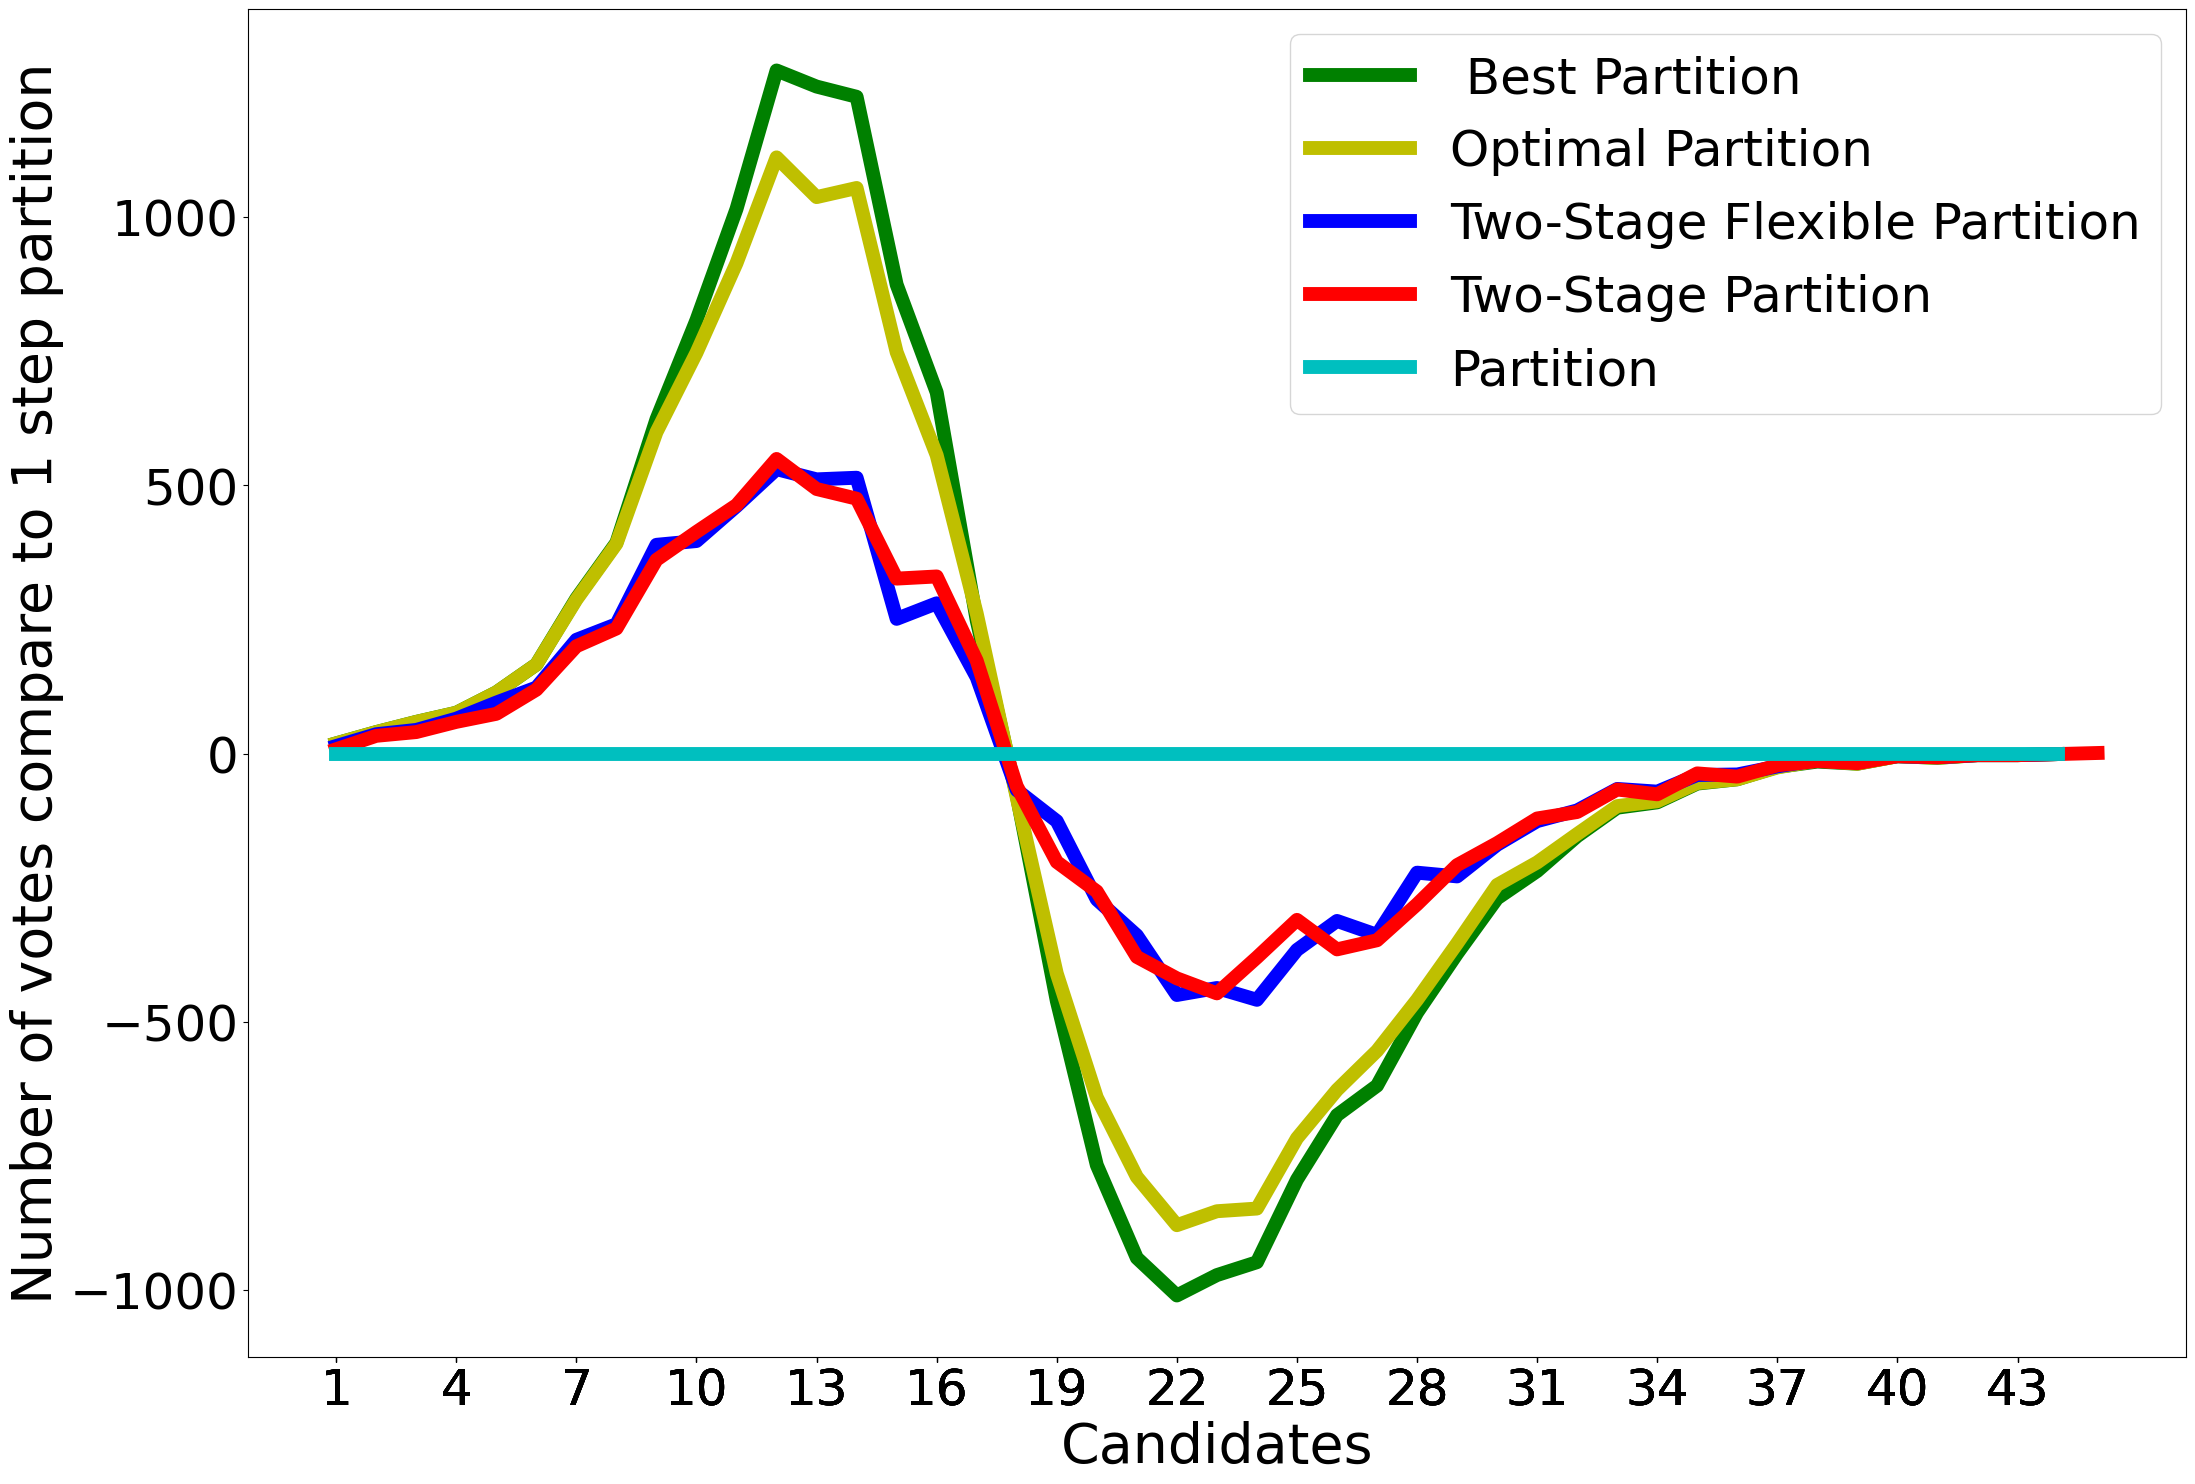
\includegraphics[width=\columnwidth]{./images/candidates_results_18_winners_phi_0_85_last_new_new_new_new.png}
\caption{Number of times each candidate has been chosen in the winning set with Best Partition, Optimal Partition, Two-Stage Flexible Partition and Two-Stage Partition compared to classic Partition as the baseline. All runs with $\phi = 0.85$, $m = 5$ and $k = 18$.}
\label{fig:candidates-performances}
\end{figure}

We see that both suggested algorithms achieved better results then the classic Partition for the same number of candidates reviewed by each agent. Figure~\ref{fig:candidates-performances} compares the candidates selected by each of the algorithms, showing that the new algorithms have a better chance of selecting middle ranking candidates from within the top-$k$ compared to classic Partition. That is, the advantage of the new algorithms is not in accepting the top agent more often (it is almost always selected by classic Partition), nor better at selecting the $k$th agent or around that (selecting more often the ($k-1$)th agent or selecting less often the ($k+1$)th agent), but rather a higher chance of selecting the $\frac{k}{2}$th agent and agents in that general ranking. In Figure~\ref{fig:recall-performance} we show that the improvement in the recall on candidates increases the noisier the information is
(i.e., as $\phi$ grows), and it is more significant the smaller the number of reviews submitted by each agent ($m$) is.
\begin{figure}[t]
\centering
\begin{subfigure}{0.8\columnwidth}
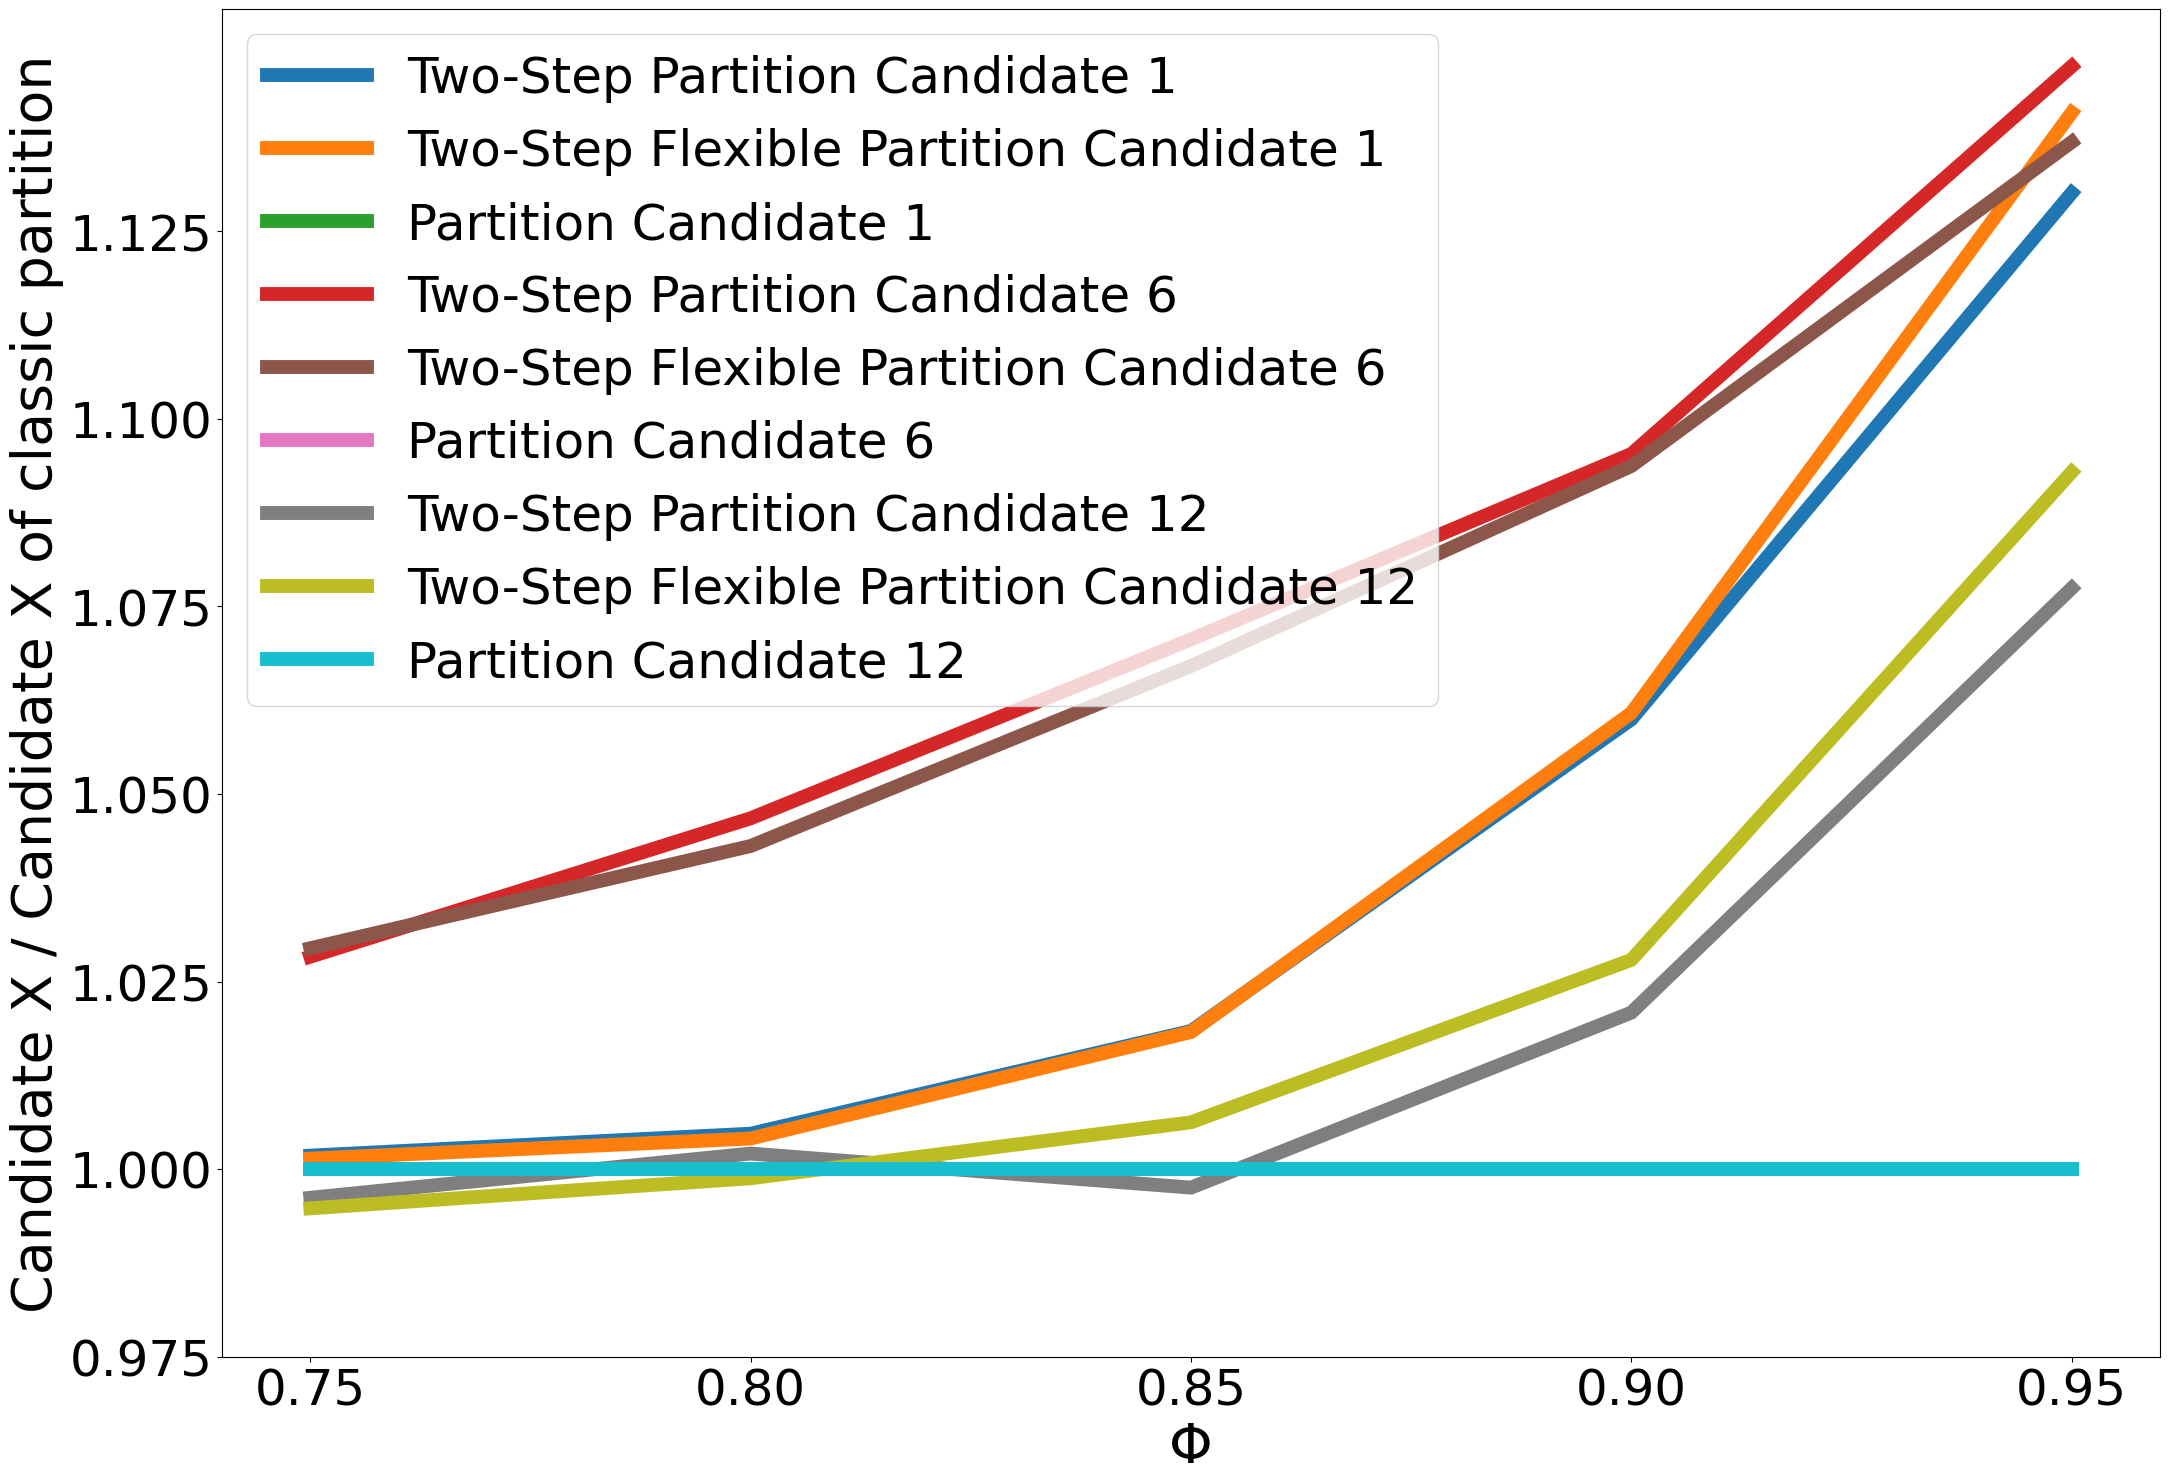
\includegraphics[width=\columnwidth]{"./images/improve_in_candidates_review_5_winner_12_new_new_new.png"}
\caption{Percent of improvement of candidate 1, candidate 6 and candidate 12 of Two-Stage Partition and Two-Stage Flexible Partition compared to 1-step Partition for different $\phi$. All runs with $m = 5$ and $k = 12$ and optimal $l$, $h$ and $f$ values.}
\label{fig:candidates-performances_per_candidates}
\end{subfigure}%
\end{figure}
Examining significance, using $\chi^{2}$ test we found that when $k= 6$, for $\phi\geq 0.7$ and $m\leq 11$, the improvement of the Two-Stage mechanisms is significant. For $k=12$, for $\phi\geq 0.75$ and $m\leq 11$, the improvement over 1-step Partition is, again, significant. For $k= 18$, for $\phi\geq 0.8$ and $m\leq 11$, the improvement is significant. This does make intuitive sense, as the larger $k$ grows, it is easier, even with mildly correlated rankings, to approximate the ground-truth. Hence, when $k$ grows, the significant results happen with a larger $\phi$, and when $m$ is large enough, even Partition can get very good results, hence the lack of significance for those values. Examining specific candidates, we see our intuition regarding Figure~\ref{fig:candidates-performances} is correct -- for example, for $k=18, m=5, \phi=0.85$, the improvement of Two-Stage Partition over regular Partition is highly significant ($p<0.001$) for candidates 3-17, very significant for candidate 2 ($p<0.005$), and still significant for candidate 1 ($p<0.05$).

\begin{figure*}
\centering
\begin{subfigure}{0.24\textwidth}
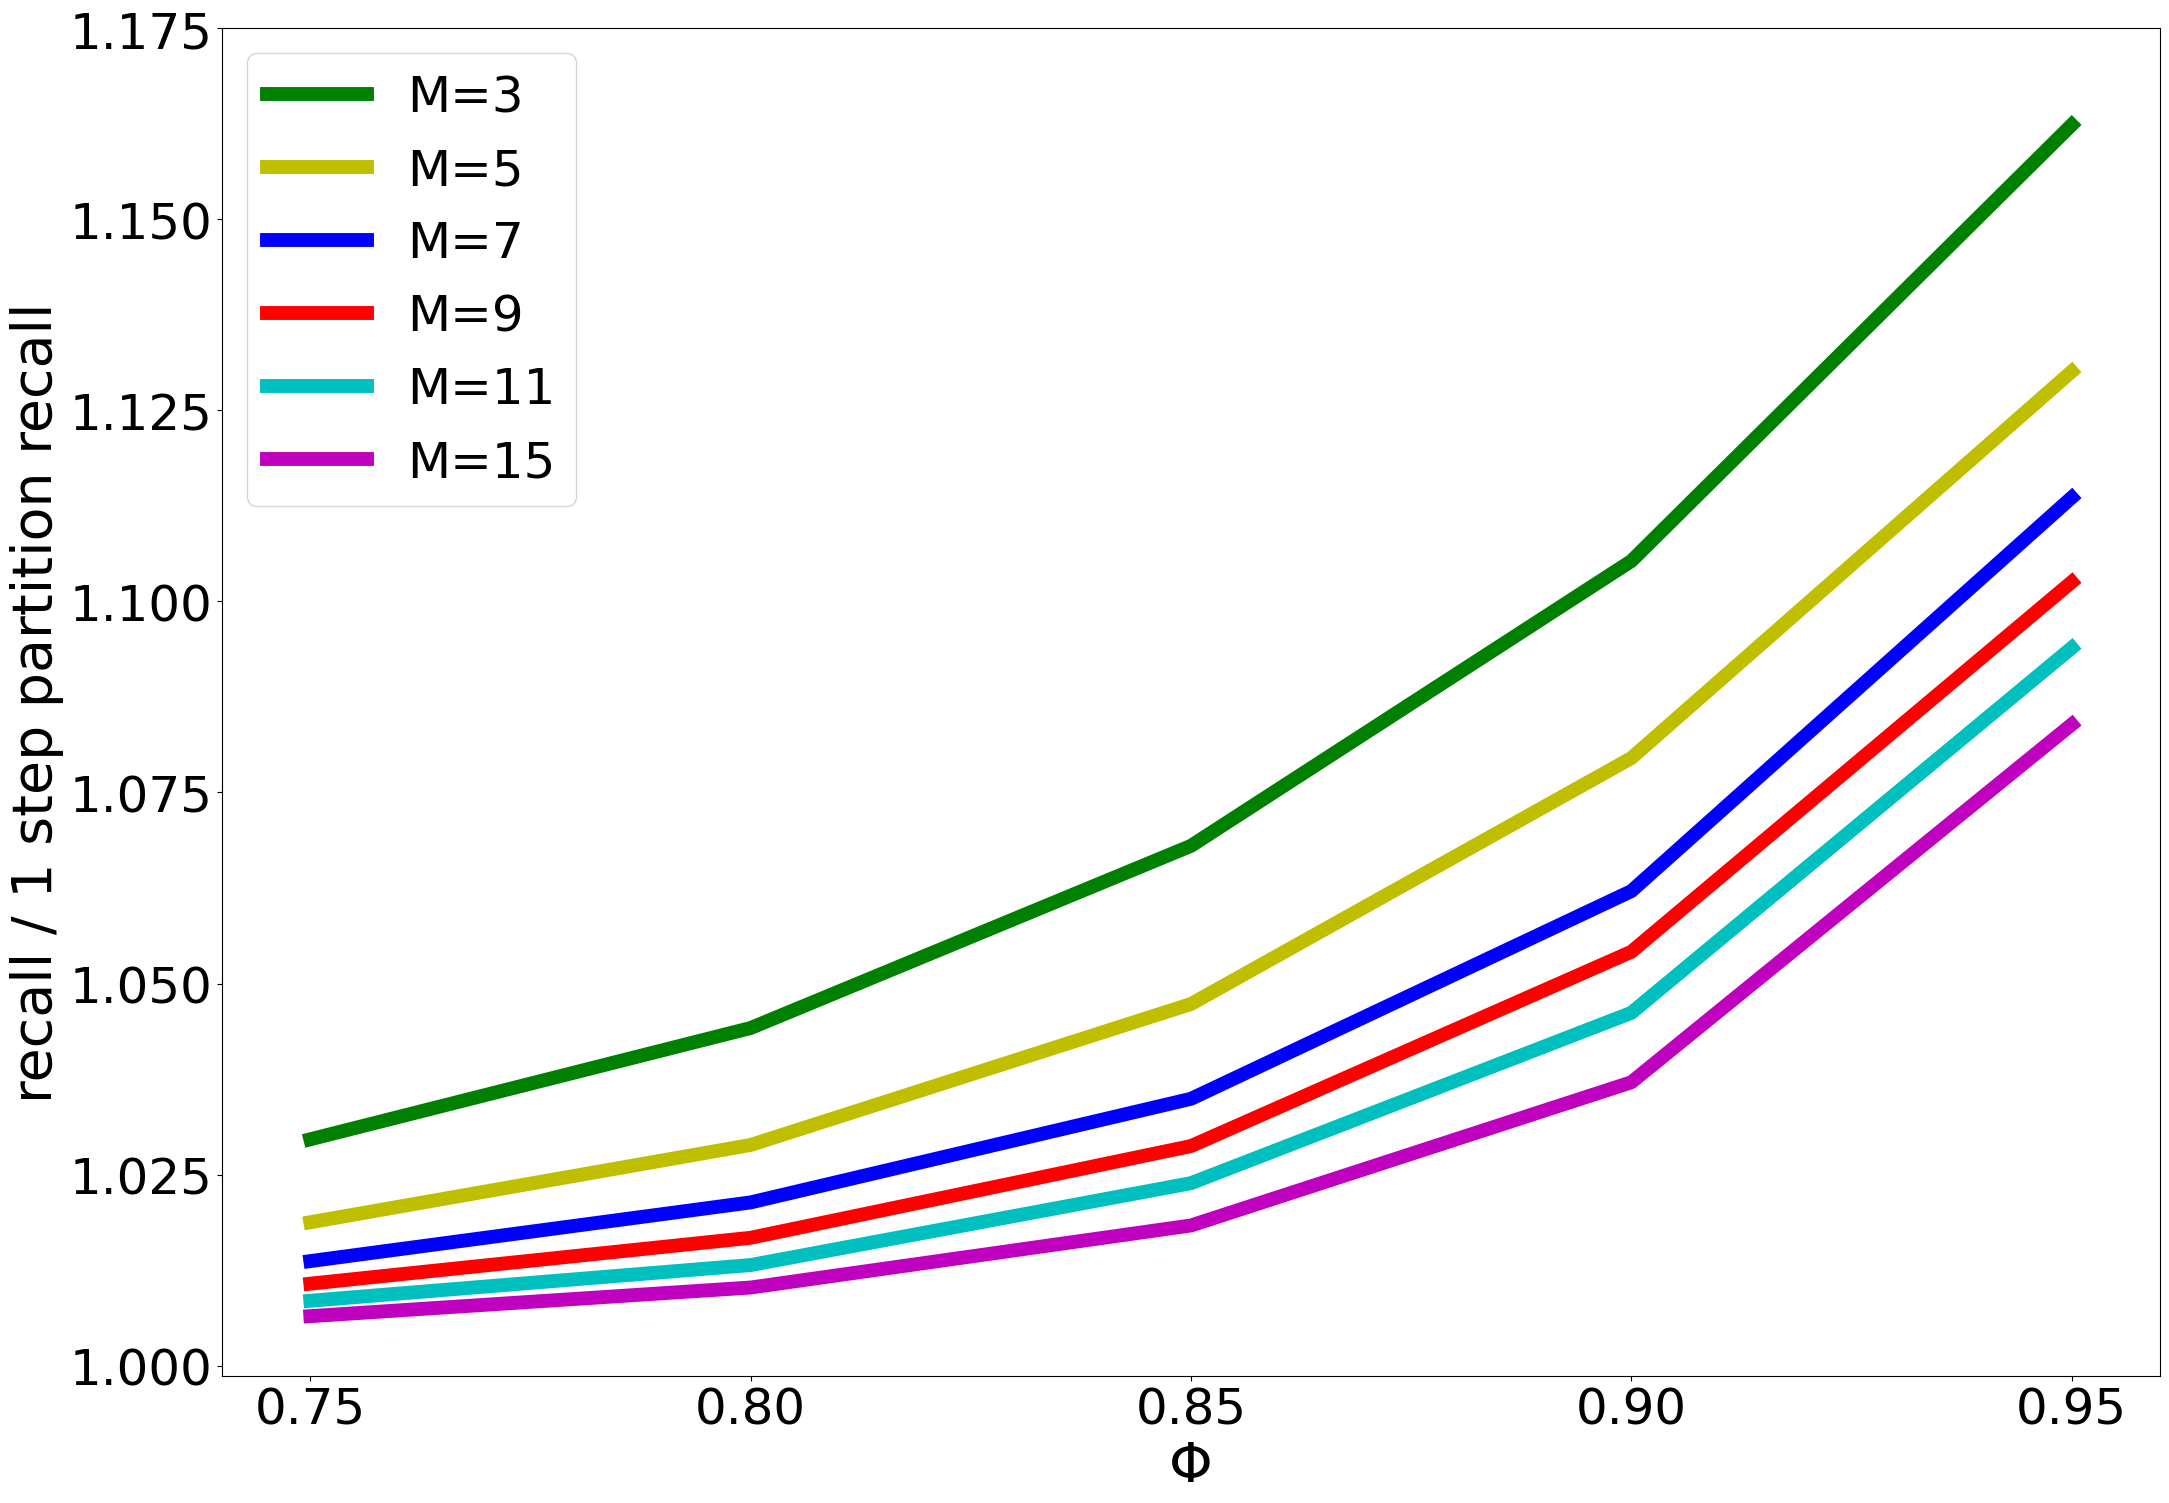
\includegraphics[width=\textwidth]{"./images/recall_compare_1_step_partition_with_phi_new_new.png"}
\caption{Two-Stage Partition compared to 1-step Partition for different $m$ and $\phi$ values. All runs with $k = 12$.}
\label{fig:recall-performance}
\end{subfigure}%
\hfill
\begin{subfigure}{0.24\textwidth}
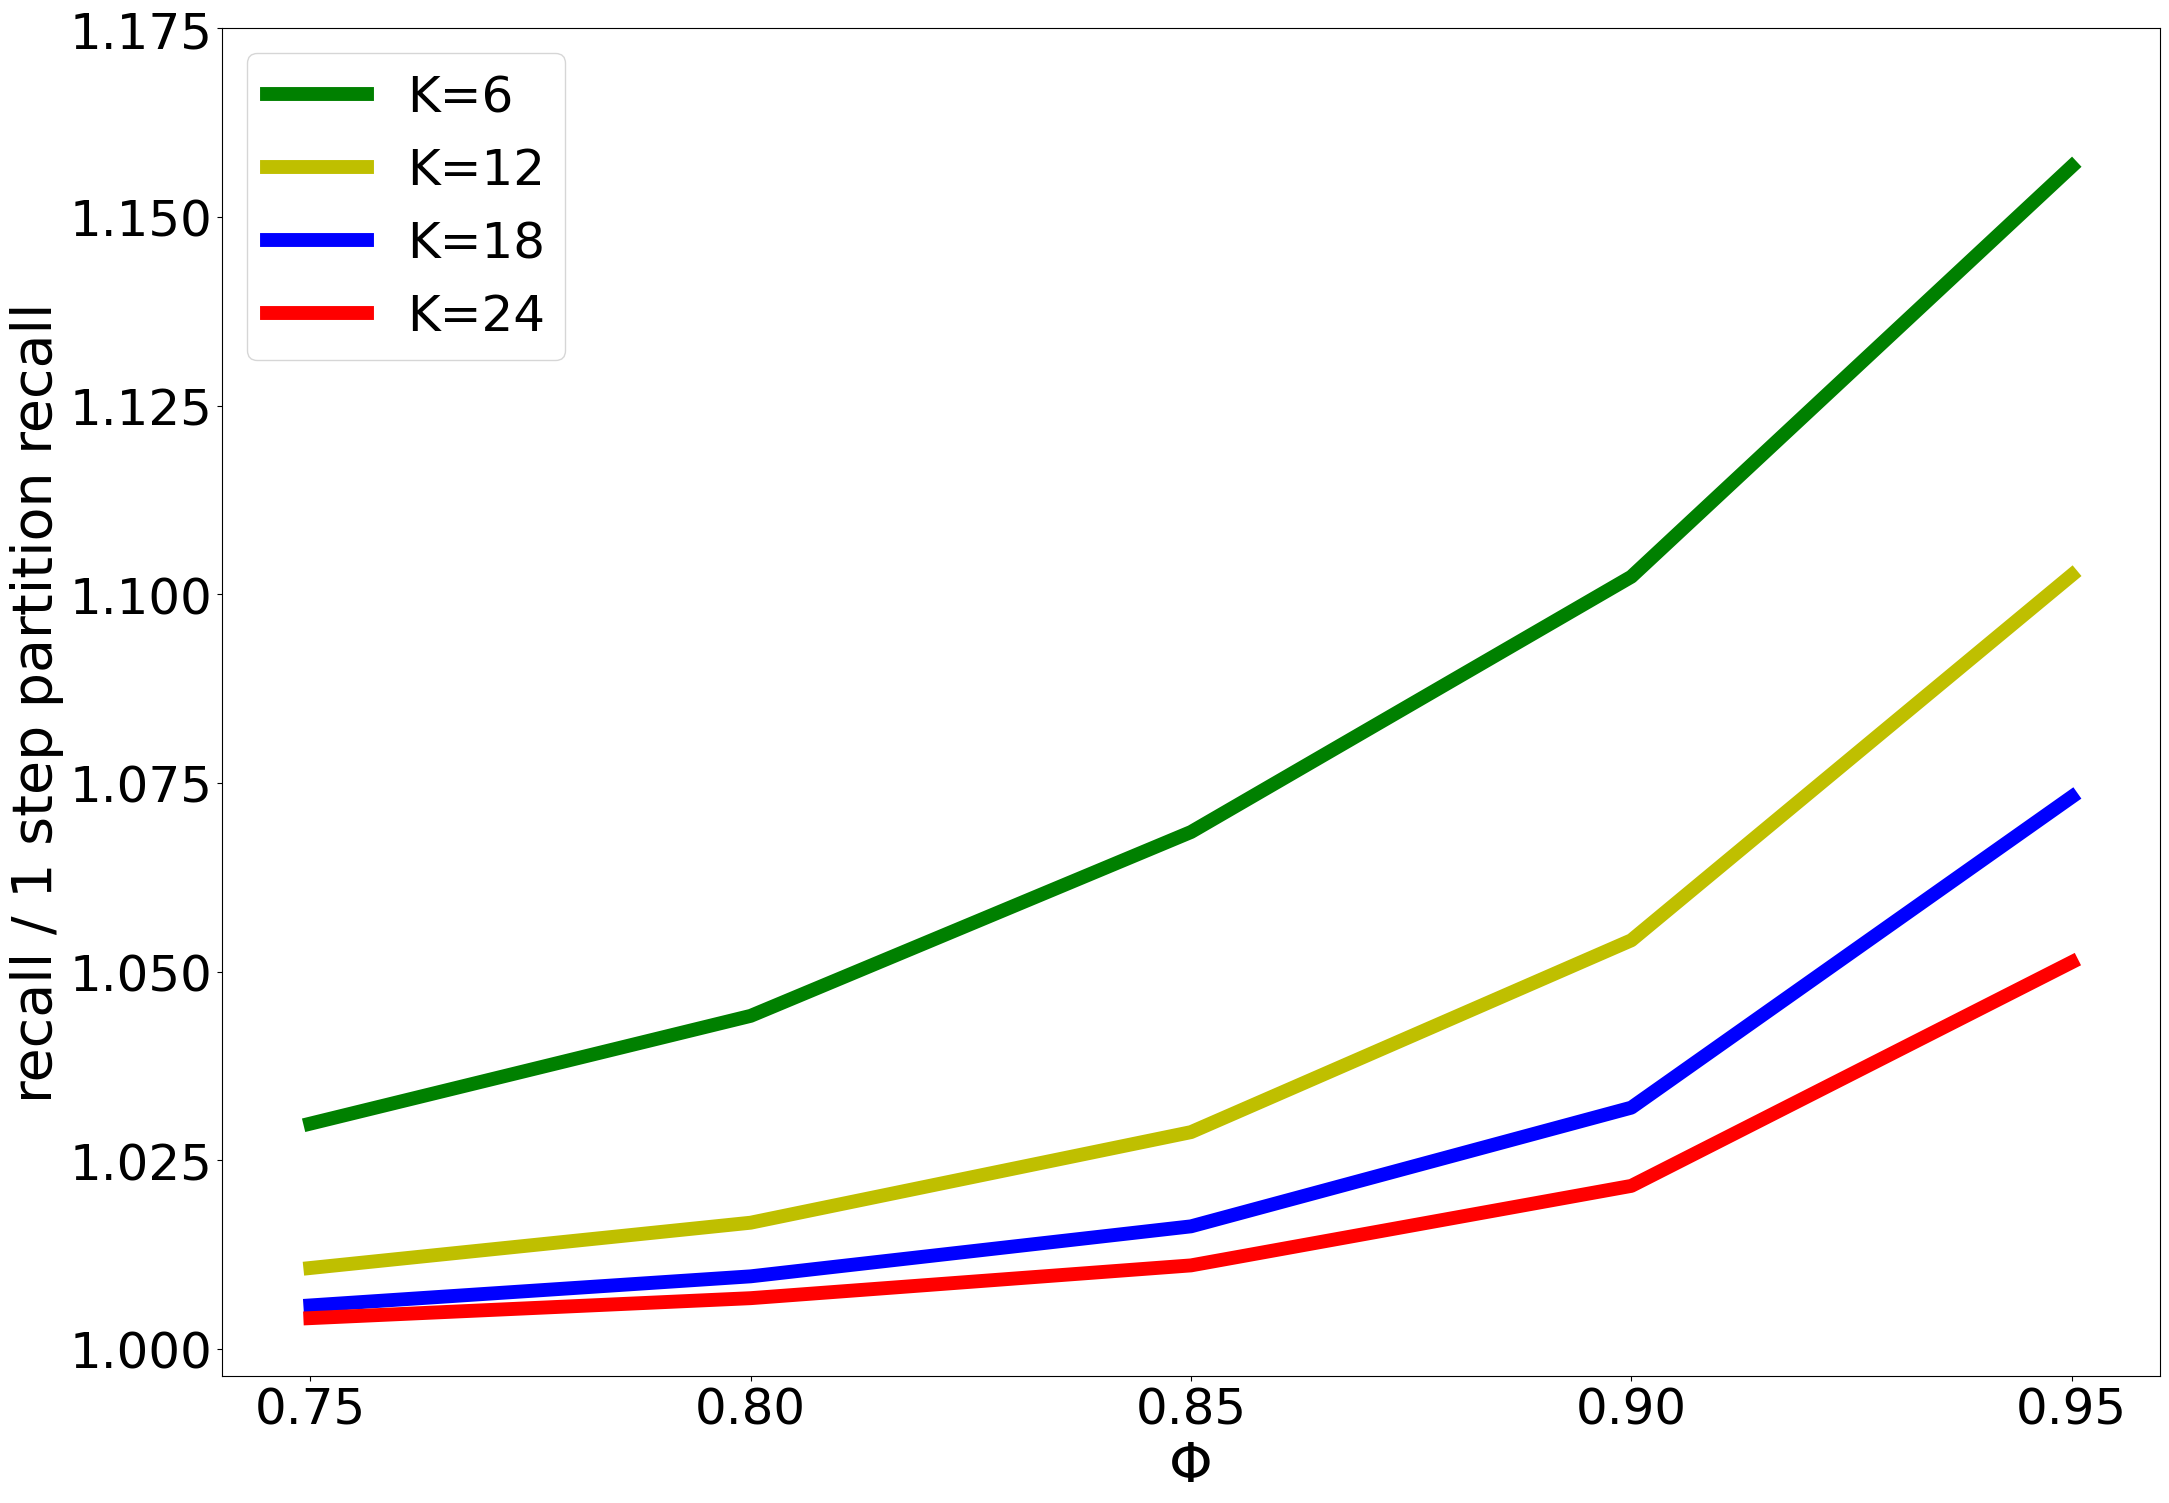
\includegraphics[width=\textwidth]{"./images/recall_compare_1_step_partition_reviews_with_phi_new_new.png"}
\caption{Two-Stage Partition compared to 1-step Partition for different $k$ and $\phi$ values. All runs with $m = 9$.}
\label{fig:recall-performance-reviews}
\end{subfigure}
\hfill
\begin{subfigure}{0.24\textwidth}
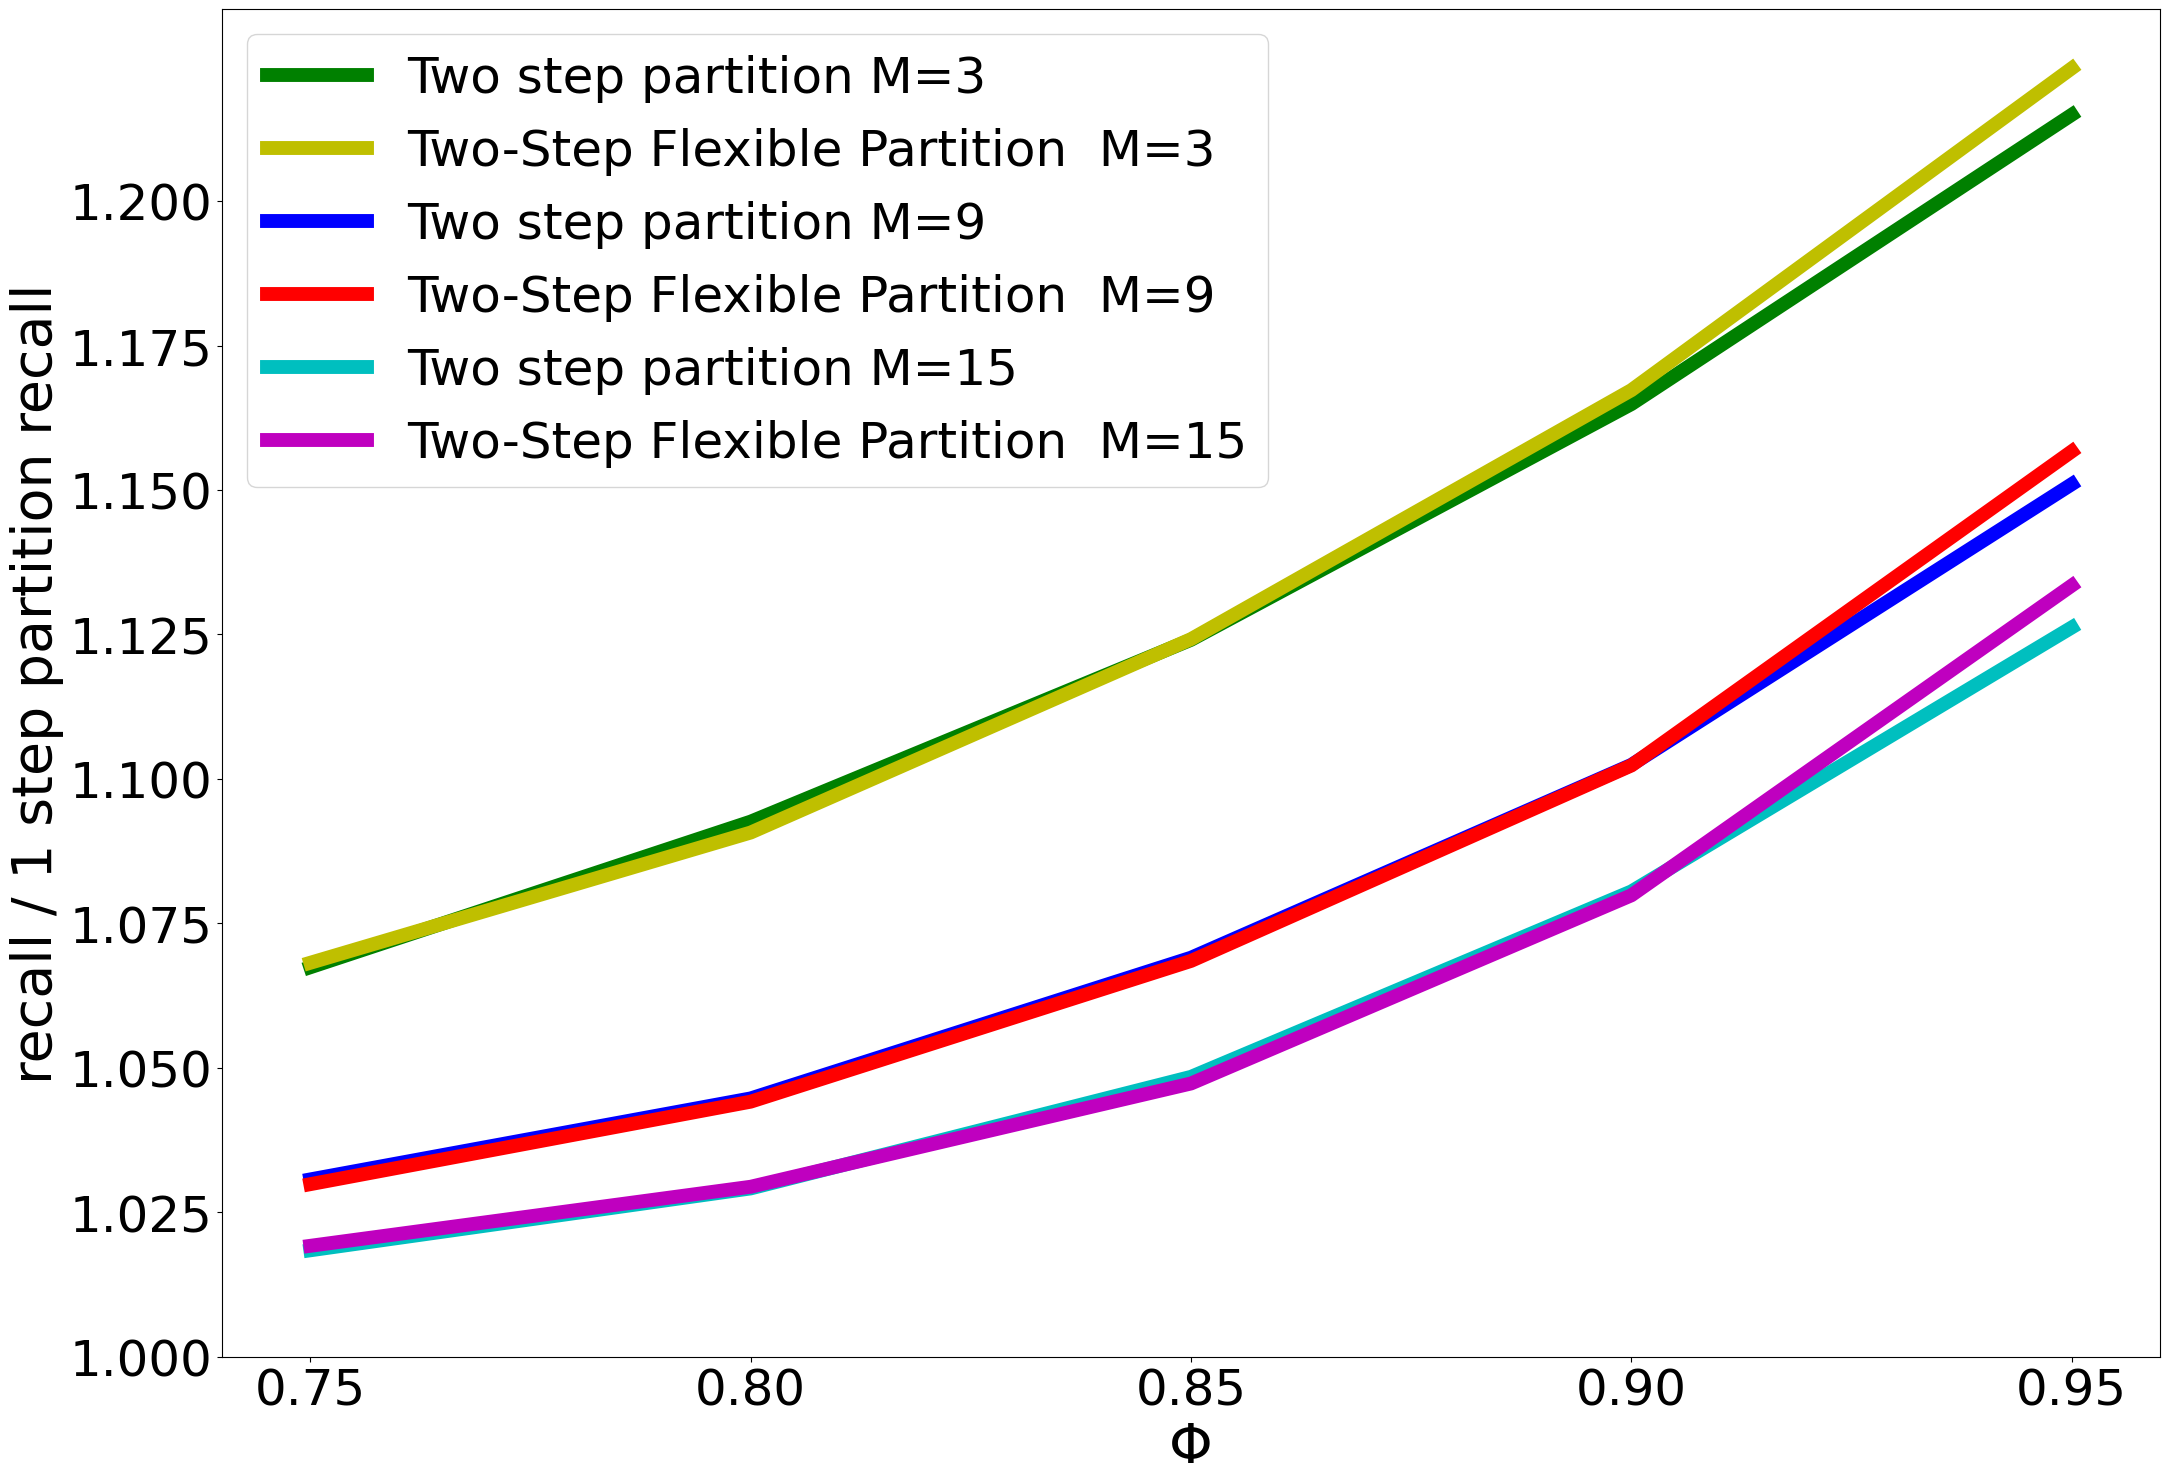
\includegraphics[width=\textwidth]{"./images/recall_compare_1_step_partition_with_phi_2_algo_new_new.png"}
\caption{Two-Stage Partition and Two-Stage Flexible Partition compared to 1-step Partition for different $m$ and $\phi$ values. All runs with $k = 18$.}
\label{fig:recall-performance-2-algo}
\end{subfigure}
\hfill
\begin{subfigure}{0.24\textwidth}
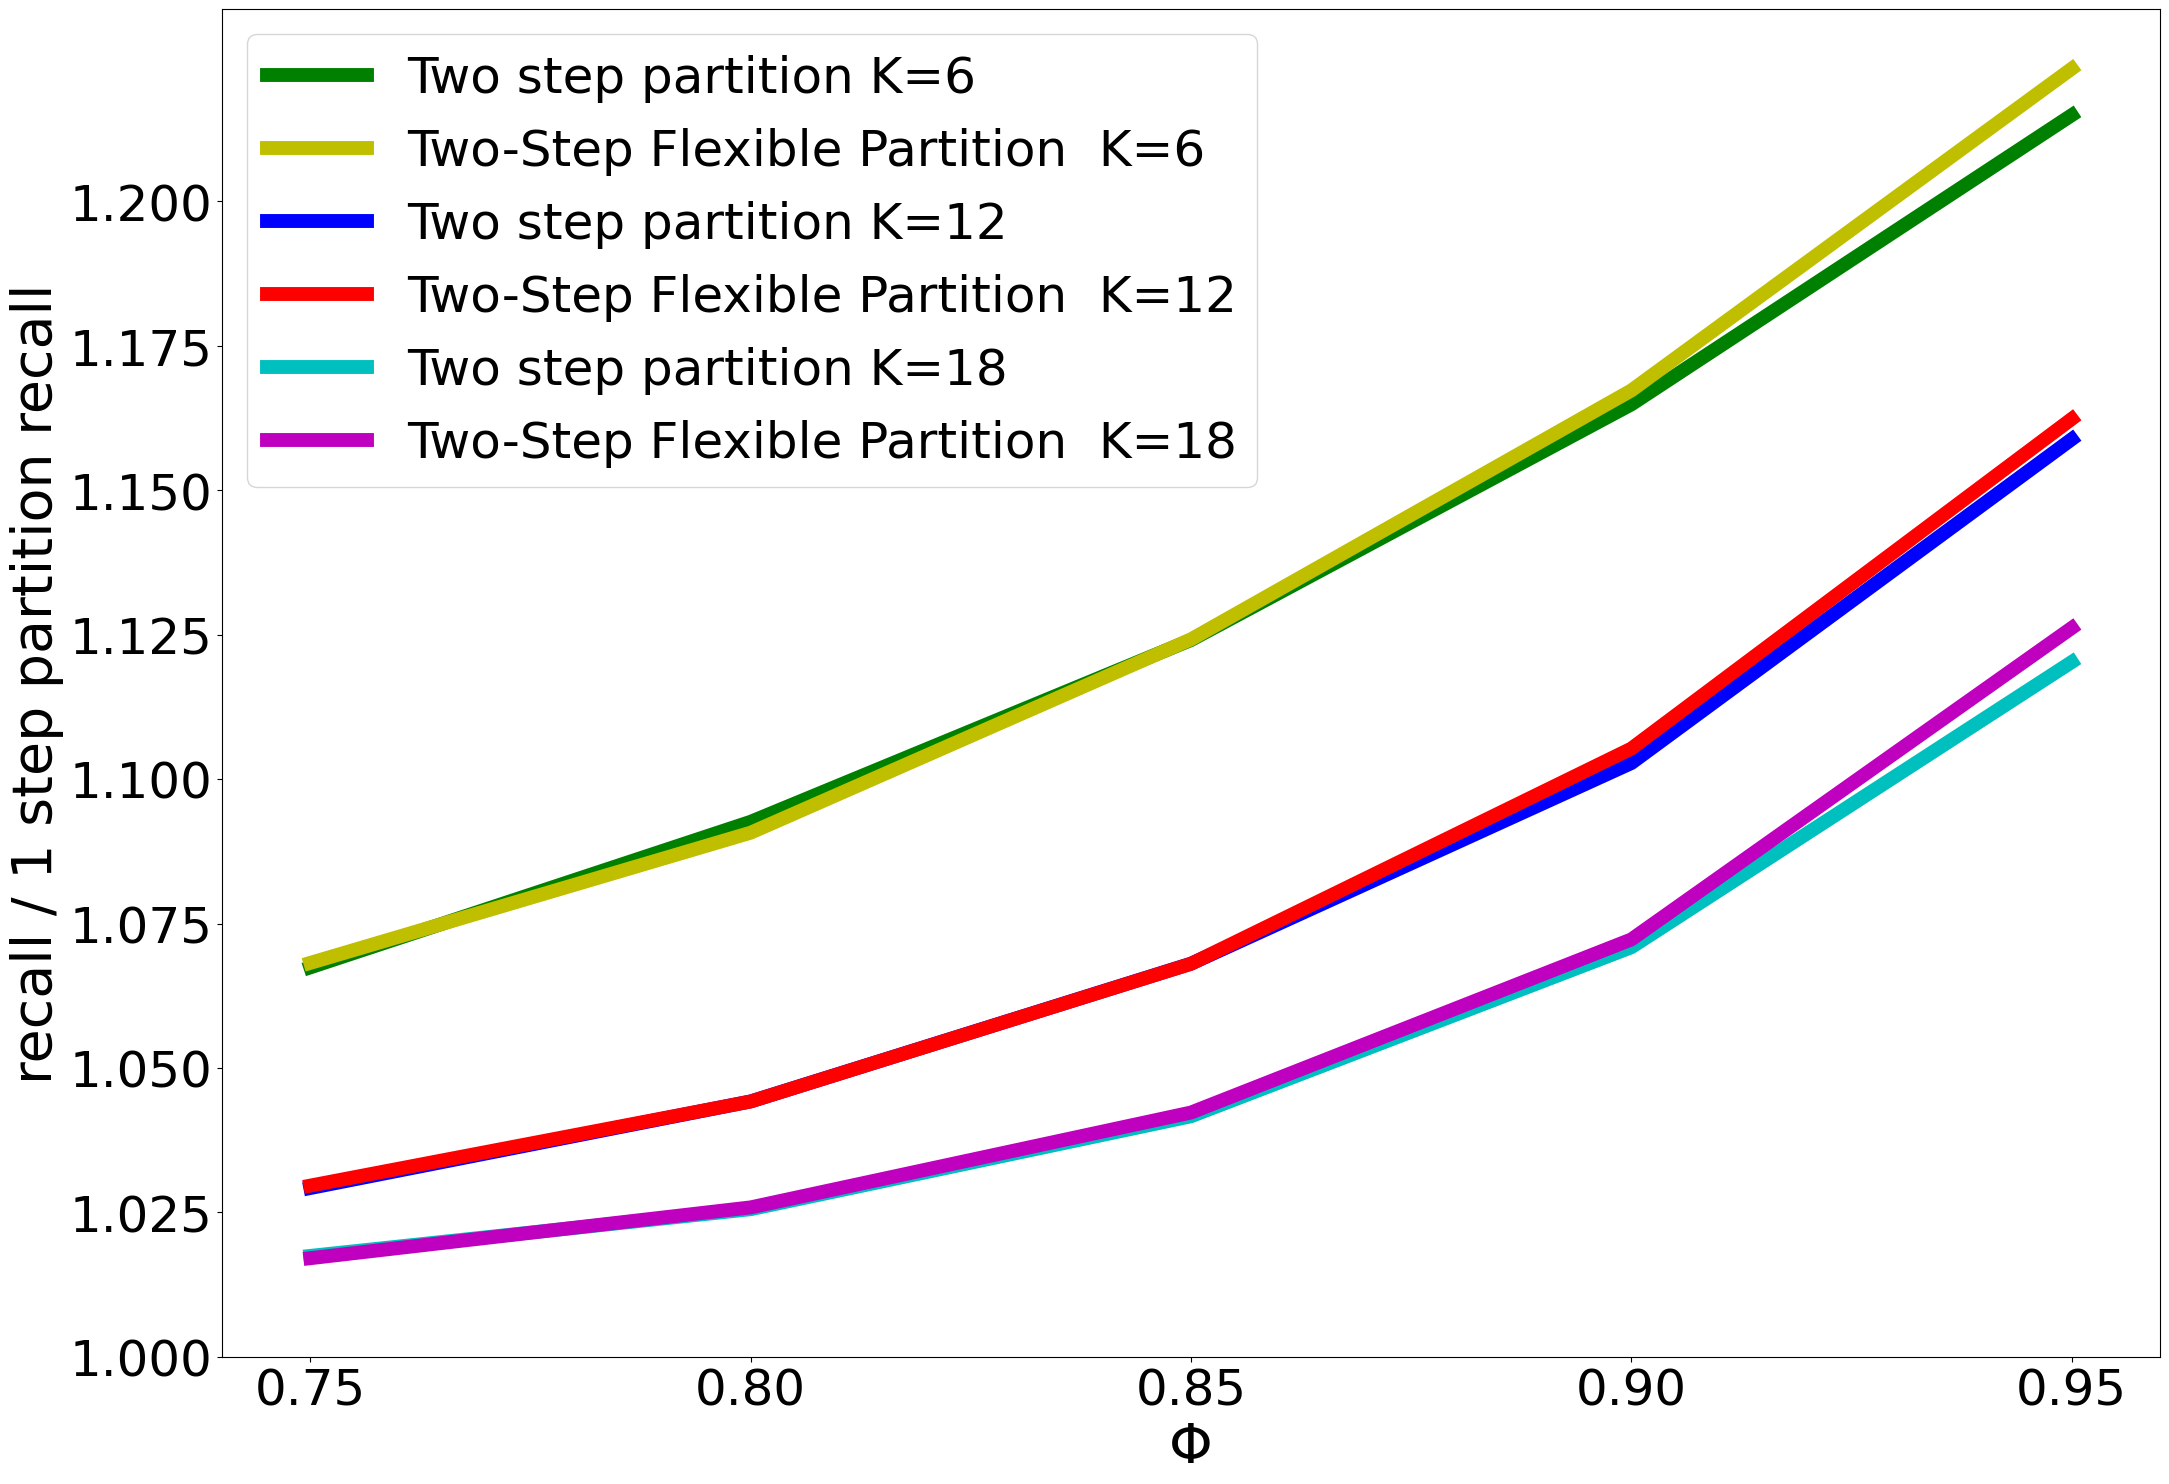
\includegraphics[width=\textwidth]{"./images/recall_compare_1_step_partition_reviews_with_phi_2_algo_new_new_new.png"}
\caption{Two-Stage Partition compared to 1-step Partition for different $k$ and $\phi$ values. All runs with $m = 3$.}
\label{fig:recall-performance-reviews-2-algo}
\end{subfigure}%

\label{fig:second}
\caption{Percent of improvement in recall compared to 1-step Partition. All runs with optimal $f$ for that $m, k,$ and $\phi$.}
\end{figure*}

Figures \ref{fig:recall-performance} and \ref{fig:recall-performance-reviews} compare the performance of the new algorithms depending on the size of the winner group ($k$), and on how many reviews are submitted by each agent ($m$). Of course, having all possible information is best, hence Partition with $\frac{n}{2}$ reviews dominates everything (but is not realistically implementable). We see that both new algorithms have a better recall than classical Partition, but when the $k$ or $m$ are small, the new algorithms have the most advantage over it. We also see a large advantage to the new algorithms when candidates' votes are more noisy, i.e., larger $\phi$.

Figure~\ref{fig:candidates-performances_per_candidates} strengthens the statement above regarding the significant contribution of the two-stage mechanisms particularly to the mid-$k$ candidates. We see that the middle candidate had the most improvement, and this advantage grew as the votes were less correlated ($\phi$ grew). Moreover, the raw numbers in Figure~\ref{fig:candidates-performances_per_candidates_in_winning_group} show that this improvement over Partition on noisy votes, i.e., higher $\phi$, is not due to a better performance on the noisy votes (unsurprisingly, it is easier to find the top $k$ when votes are close to ground-truth), but rather due to a larger improvement over Partition, which becomes worse much faster in noisy settings.

When comparing the two new suggested algorithms, we find that the algorithms' fine-tuning parameters (e.g., size of $f$, etc.) are quite similar for both. But we see that when votes are less noisy, i.e, smaller $\phi$, there is a slight advantage to Two-Stage Partition, and when votes are more noisy, i,e., larger $\phi$, Two-Stage Flexible Partition has a slight advantage. This seems to imply that the flexibility of Two-Stage Flexible Partition does indeed come to play with noisy rankings, and is able to correct for a mediocre first round. Figures \ref{fig:recall-performance-2-algo} and \ref{fig:recall-performance-reviews-2-algo} compare between the improvement of the new algorithms over regular, 1-stage, Partition depending on the size of the winner group ($k$) and on the number of reviews ($m$). We see that as $k$ grows and $m$ is smaller, Two-Stage Flexible Partition achieves better results compared to Two-Stage Partition. This might be explained, as before, as higher $k$ and lower $m$ are more sensitive to errors with uncorrelated preferences (larger $\phi$), making the flexibility meaningful.

\subsection{Algorithm Fine-Tuning}

\begin{figure}[t]
\centering
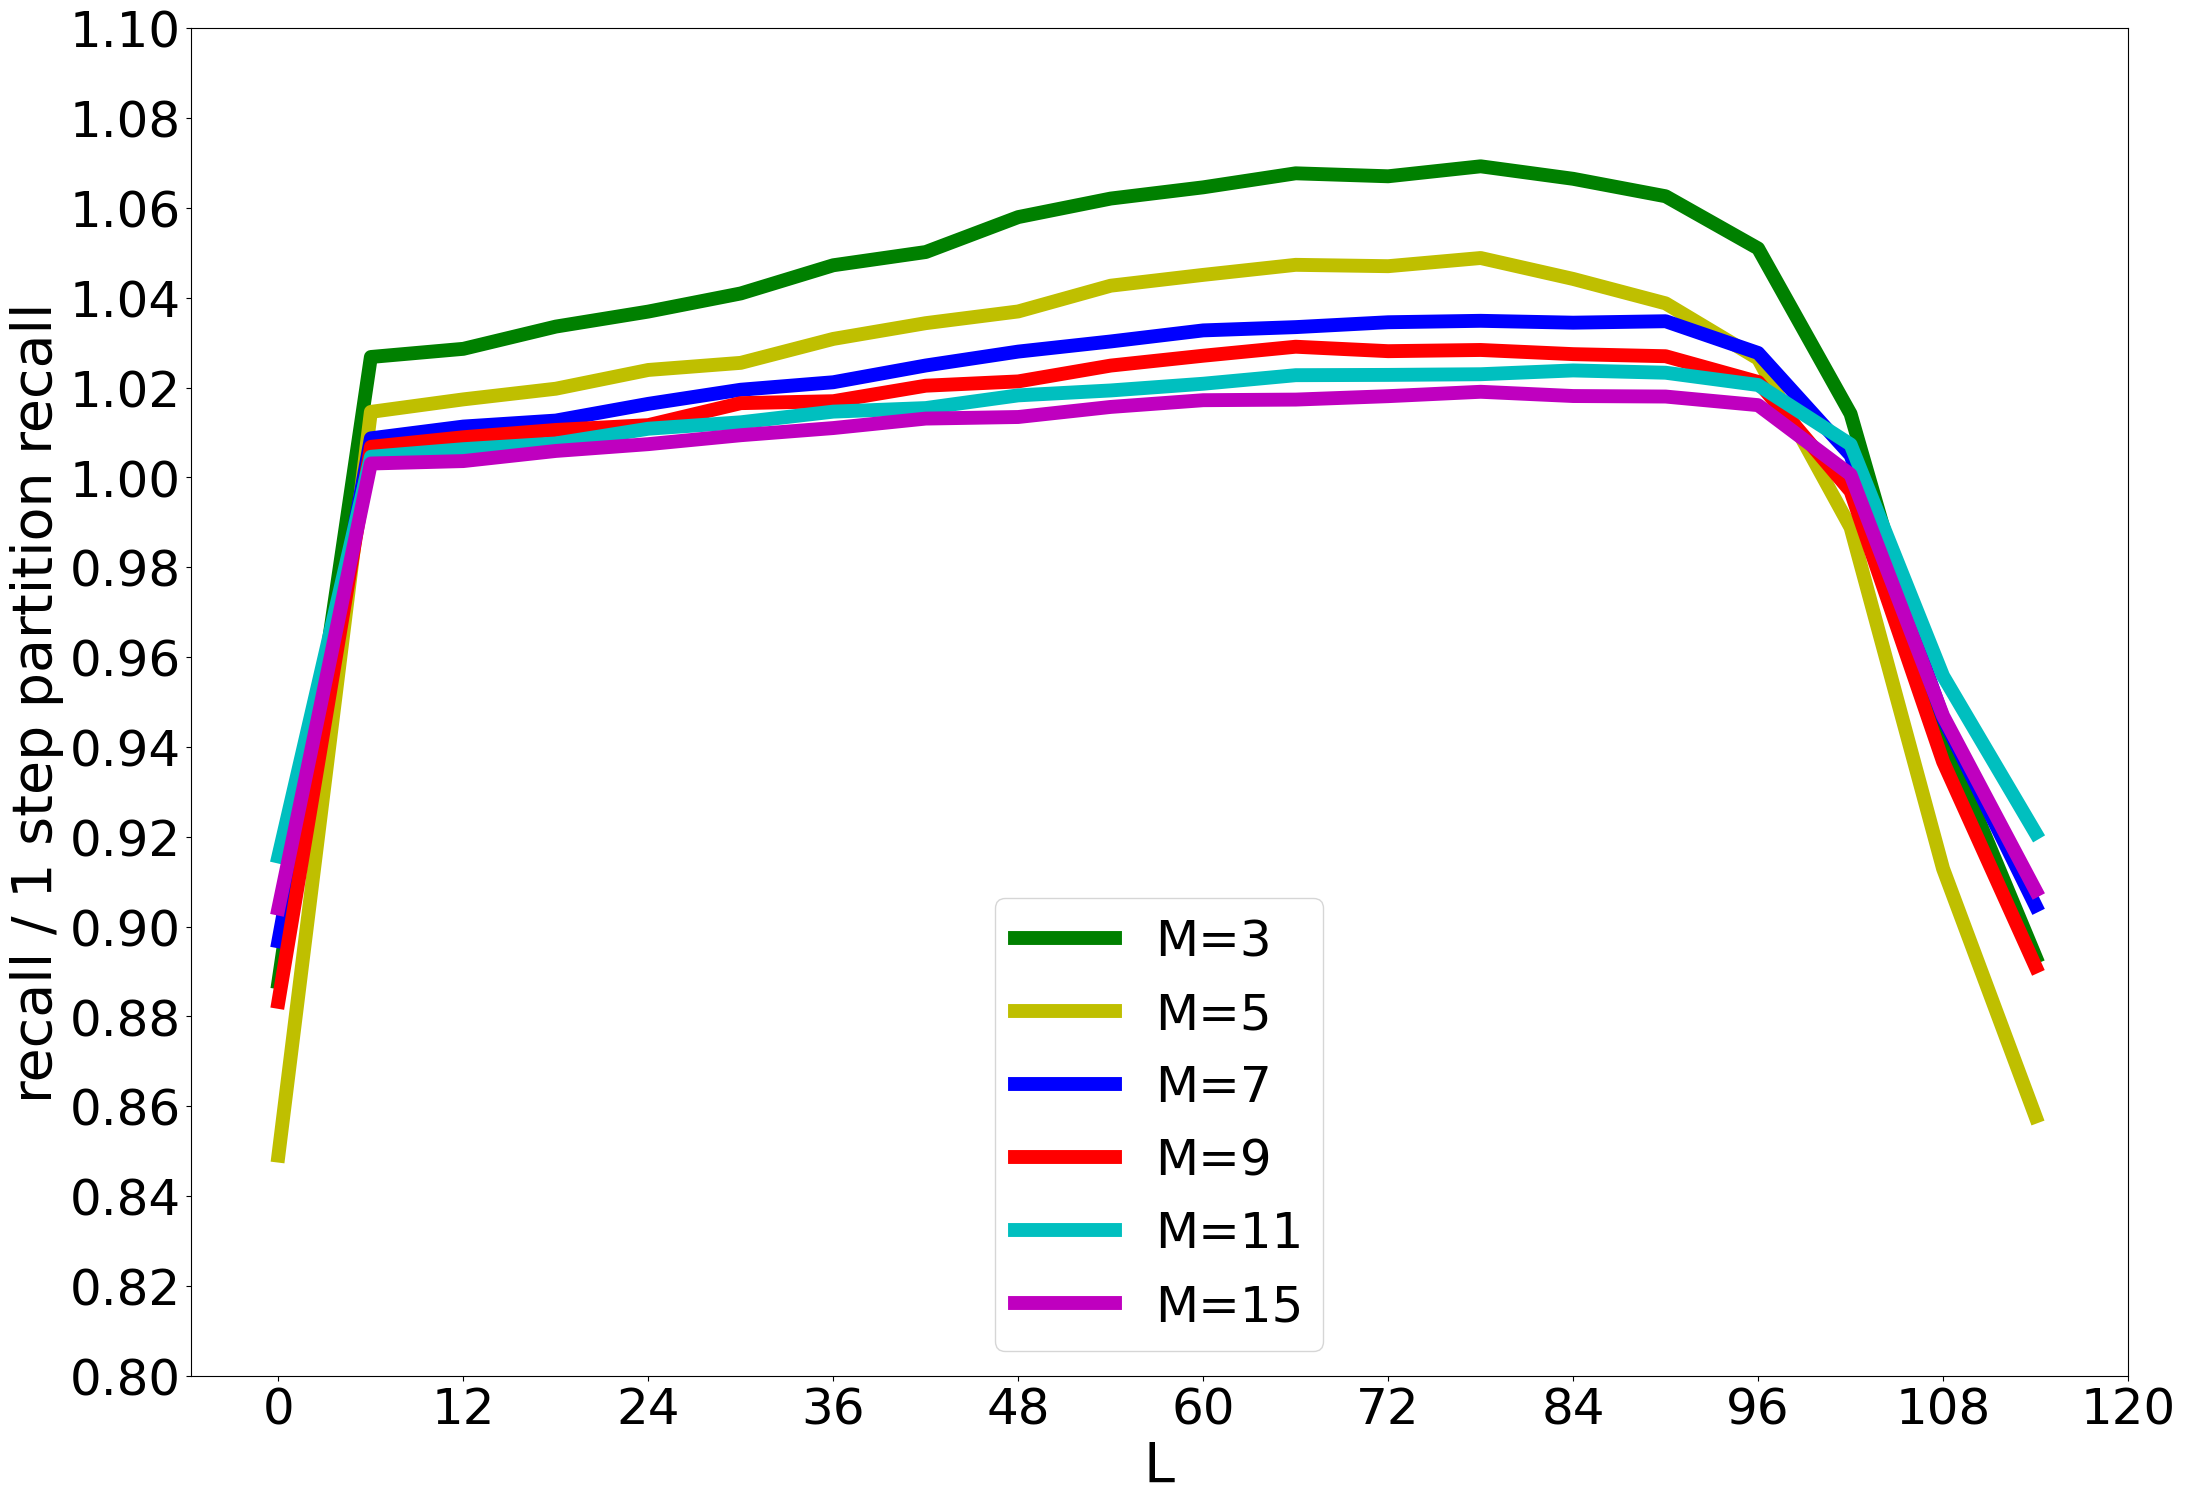
\includegraphics[width=0.8\columnwidth]{./images/First_step_loser_phi_0_85_split_per_0_2_win_group_0_m_12_new.png}
\caption{Percent of improvement of Two-Stage Partition recall over 1-step partition, for different values of $l$. All runs with $\phi = 0.85$, $k = 12$, $f = \frac{2m}{10}$, $h = 0$.}
\label{fig:First_step_loser_change}
\end{figure}

We now examine the various parameters and see which values lead the Two-Stage Partition mechanisms to their best performance (as noted above, both algorithms are similar with regard to their optimal parameter choice). To do so, we wish to find when Two-Stage Partition recall was closest to regular Partition with everyone reviewing everyone else (Optimal Partition). Note that we are not comparing to the ground truth, as we wish to compare to the best information that is possible to glean from all possible reviews.



We assume $\phi$, $k$ and $m$ are given as part of the problem description (e.g., peer evaluation of students in an online course may have higher $\phi$ than scientific conference reviews). In contrast to those, $f$, $h$ and $l$ are parameters that we can control and we can choose the best values for them given a task.



\begin{figure*}
\centering
\begin{subfigure}{0.24\textwidth}
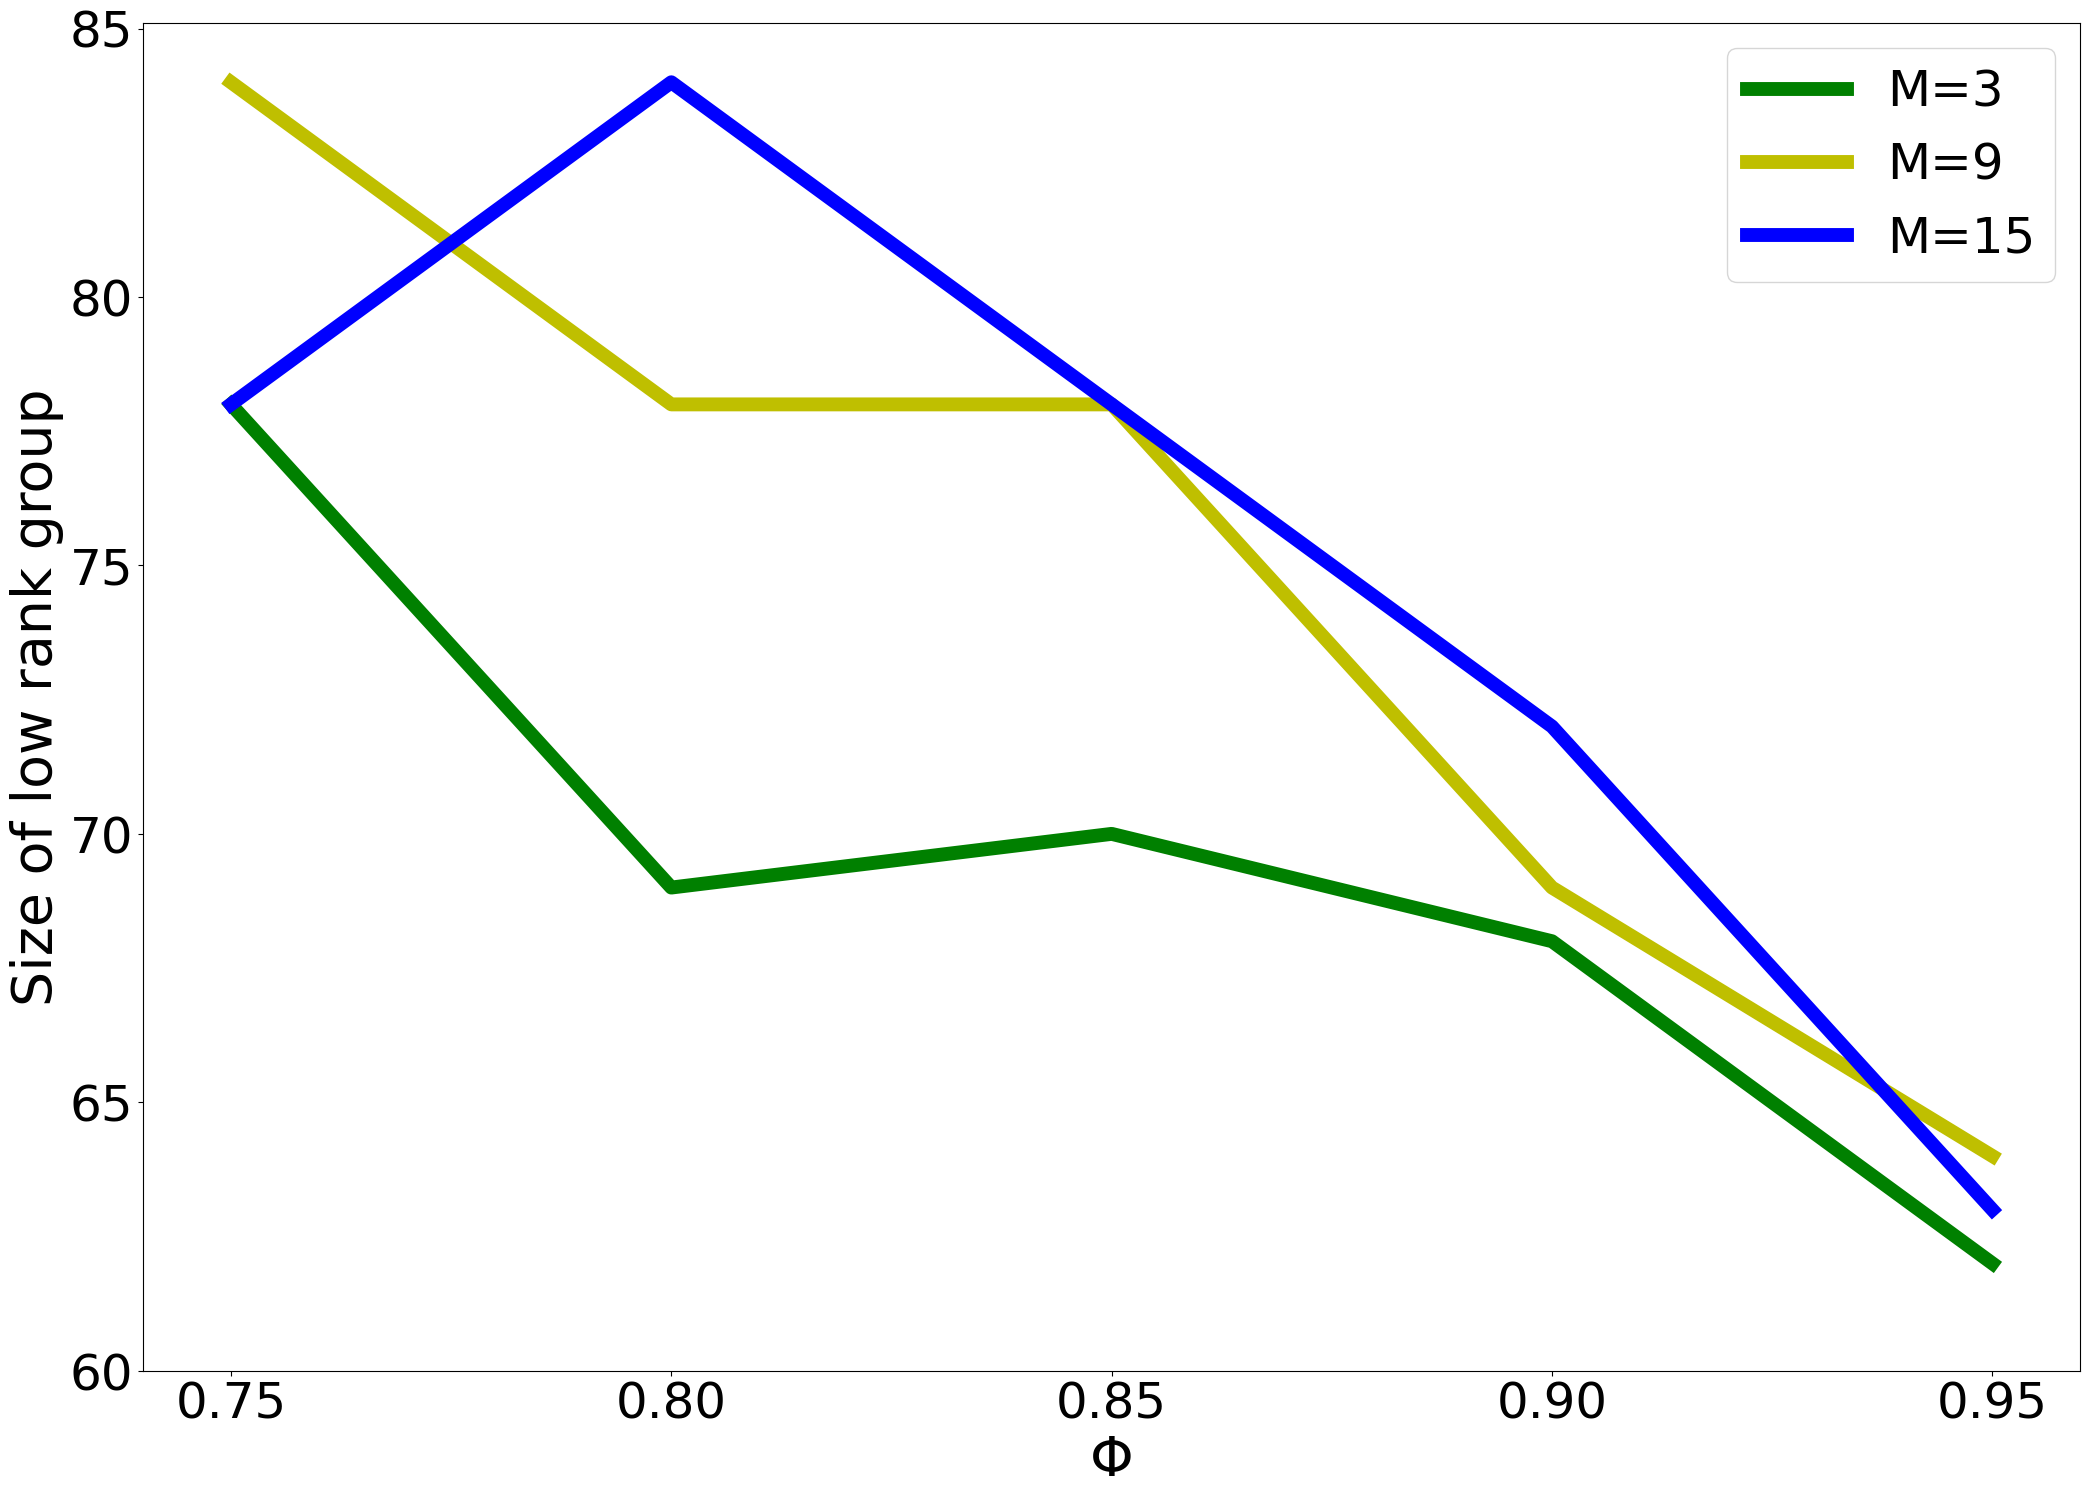
\includegraphics[width=\textwidth]{"./images/percentage_of_low_rank_group_for_num_of_winners_with_phi_new_new.png"}
\caption{Best performing size of $l$ (bottom-ranked set size) for different $m$ and $\phi$ values. All runs with $k = 18$.}
\label{fig:percentage_of_low_rank_group_for_num_of_winners}
\end{subfigure}
\hfill
\begin{subfigure}{0.24\textwidth}
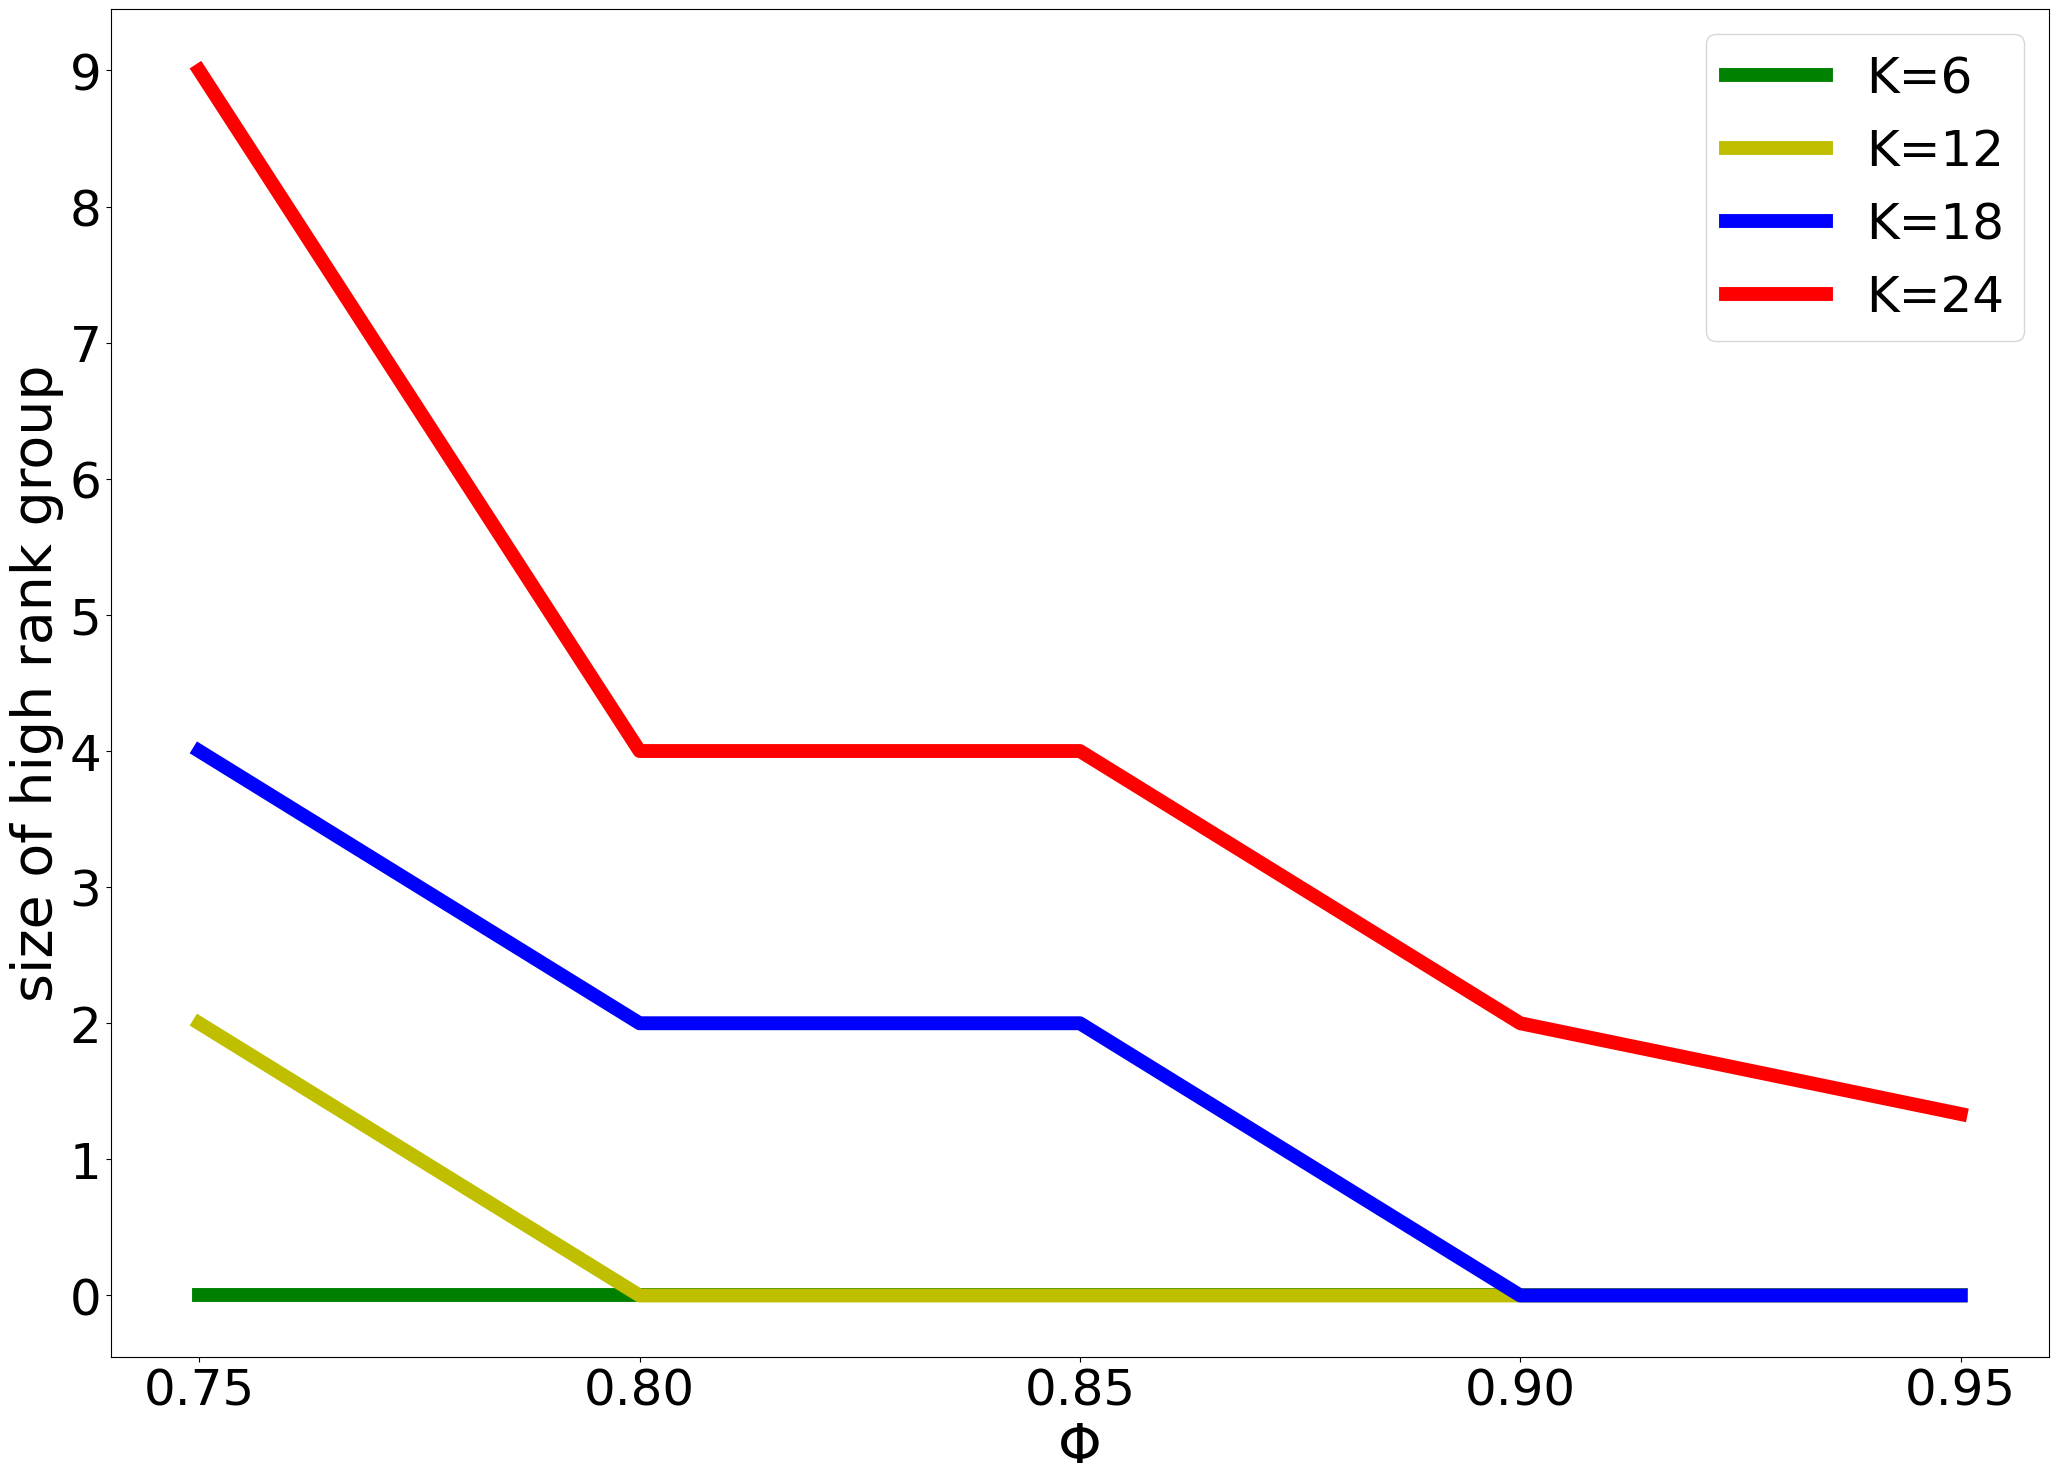
\includegraphics[width=\textwidth]{"./images/size_of_high_rank_group_for_num_of_reviews_with_phi_new_new.png"}
\caption{Best performing size of $h$ (top-ranked set size) for different $k$ and $\phi$ values. All runs with $m = 15$.}
\label{fig:size_of_high_rankk_group_for_num_of_reviews}
\end{subfigure}
\hfill
\vspace{-1.50mm}
\vspace{-1.50mm}
\vspace{-1.50mm}
\begin{subfigure}{0.24\textwidth}
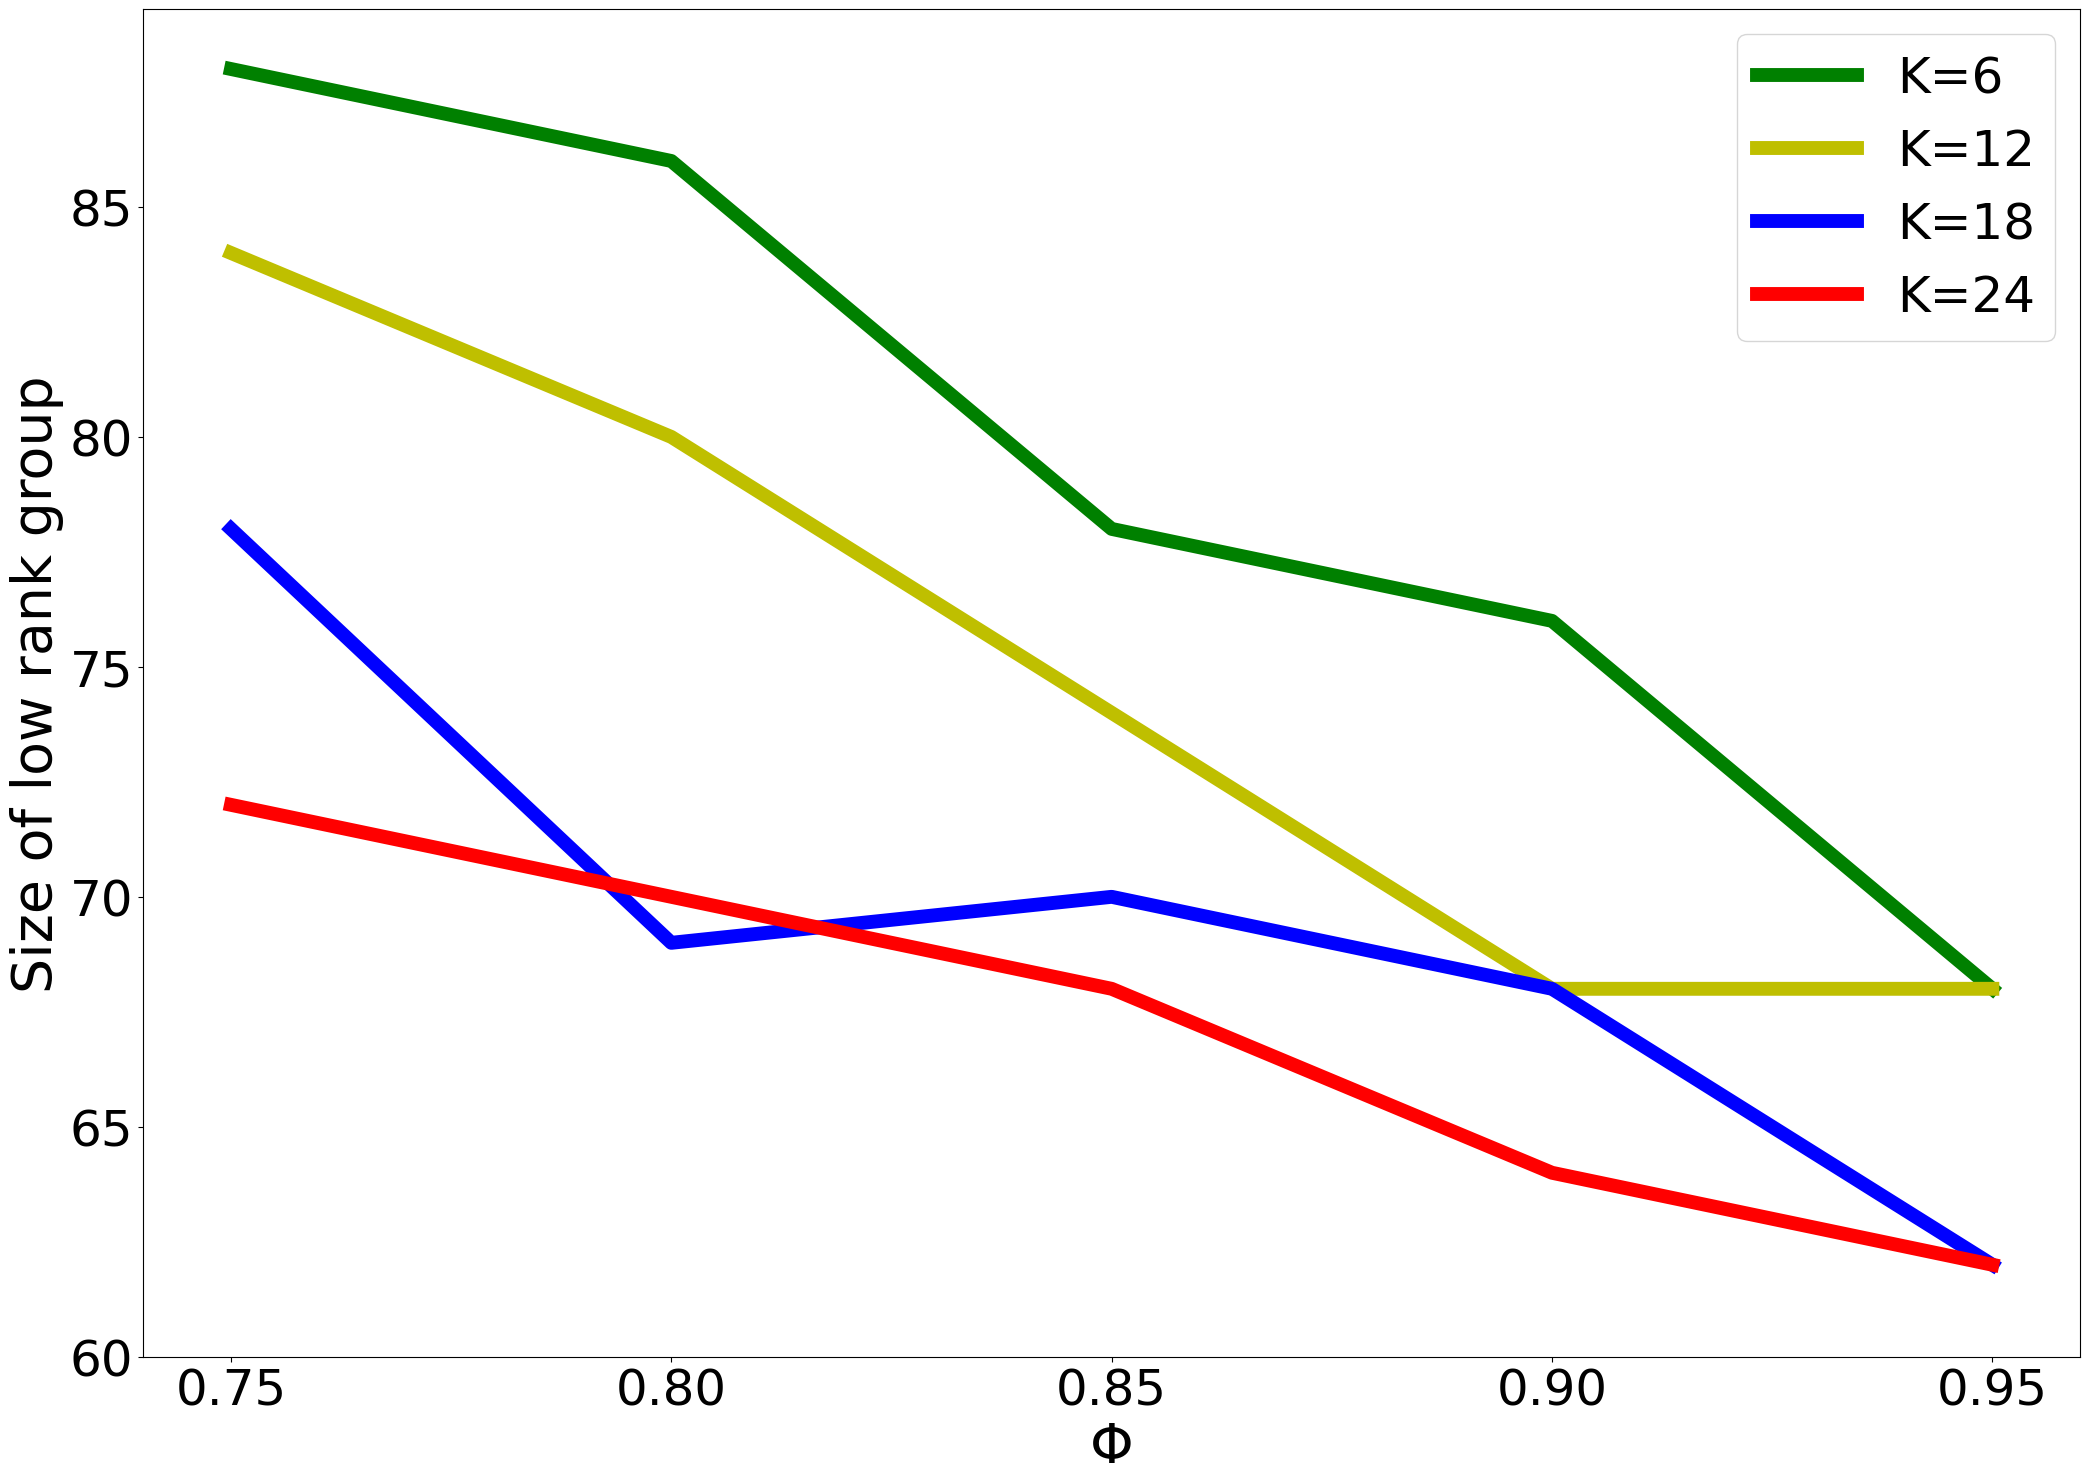
\includegraphics[width=\textwidth]{"./images/percentage_of_low_rank_group_for_num_of_reviews_with_phi_new_new.png"}
\caption{Best performing size of $l$ (bottom-ranked set size) for different $k$ and $\phi$ values. All runs with $m = 3$.}
\label{fig:percentage_of_low_rank_group_for_num_of_reviews}
\end{subfigure}
\hfill
\begin{subfigure}{0.24\textwidth}
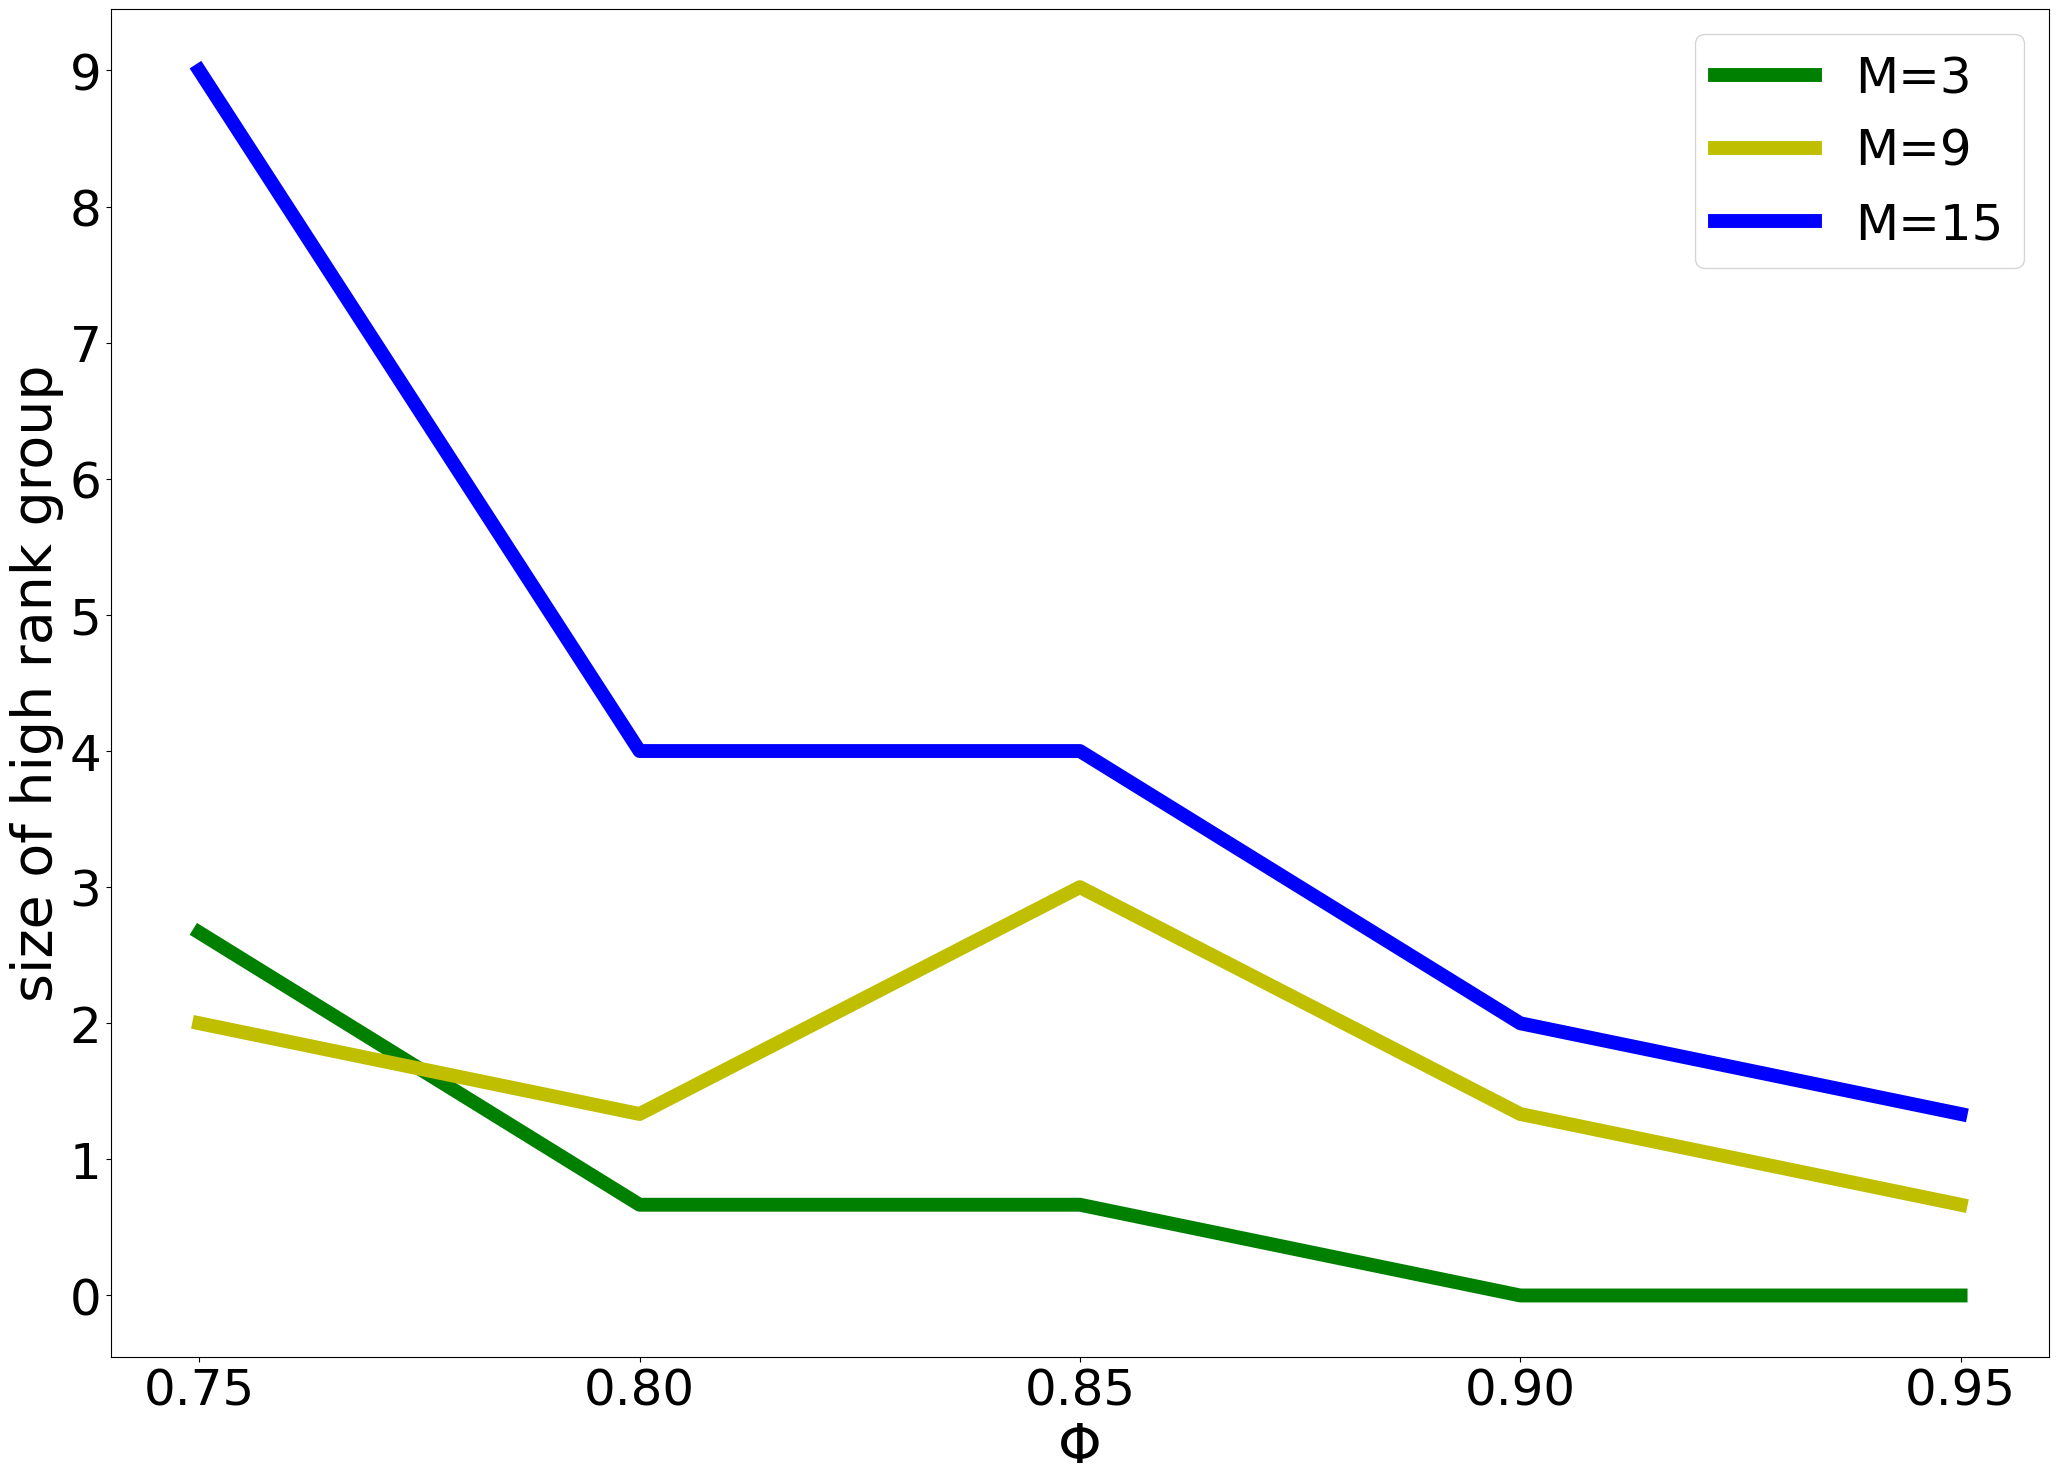
\includegraphics[width=\textwidth]{"./images/size_of_high_rank_group_for_num_of_winners_with_phi_new_new.png"}
\caption{Best performing size of $h$ (top-ranked set size) for different $m$ and $\phi$ values. All runs with $k = 24$.}
\label{fig:size_of_high_rank_group_for_num_of_winners}
\end{subfigure}
\label{fig:third}
\caption{Best performing size of top/bottom set for different values. All runs with optimal $f$ for that $m, k,$ and $\phi$.}
\end{figure*}


It seems that $f$ (the number of reviews given in the first round) should to be pretty low ($\lceil\frac{2m}{10}\rceil$), as leads to better results in all our settings (see Figure~\ref{fig:split_per_changes}). For $h$ and $l$ we see values change according to the scenario. For $l$ (the size of the group of candidates we eliminate after the first stage), we see that is better to drop a large number of candidates after first round, ideally will be in range of $\frac{n}{2}$ to $\frac{3}{4}n$ candidates, with the precise value depending on the precise values of $\phi$, $k$ and $m$ (see Figure~\ref{fig:First_step_loser_change}). When $k$ is smaller, a higher $l$ seems to work better (as can seen in Figure~\ref{fig:percentage_of_low_rank_group_for_num_of_reviews}), perhaps because when we choose fewer candidates there is less likelihood they will end up in the bottom $\frac{3}{4}n$ after the first round, and as number of winners increase we need to be more cautious about those we eliminate. We found that higher $\phi$ values will lead to lower $l$ values, probably since when reviewers are more noisy we also need be more cautious about the amount of data we use to eliminate agents. When $m$ is large, a larger $l$ works better (as can seen in Figure~\ref{fig:percentage_of_low_rank_group_for_num_of_winners}), probably because the significant number of reviews means we have enough information about the candidate even from the first stage, allowing us to eliminate with confidence.
\begin{figure}[t]
\centering
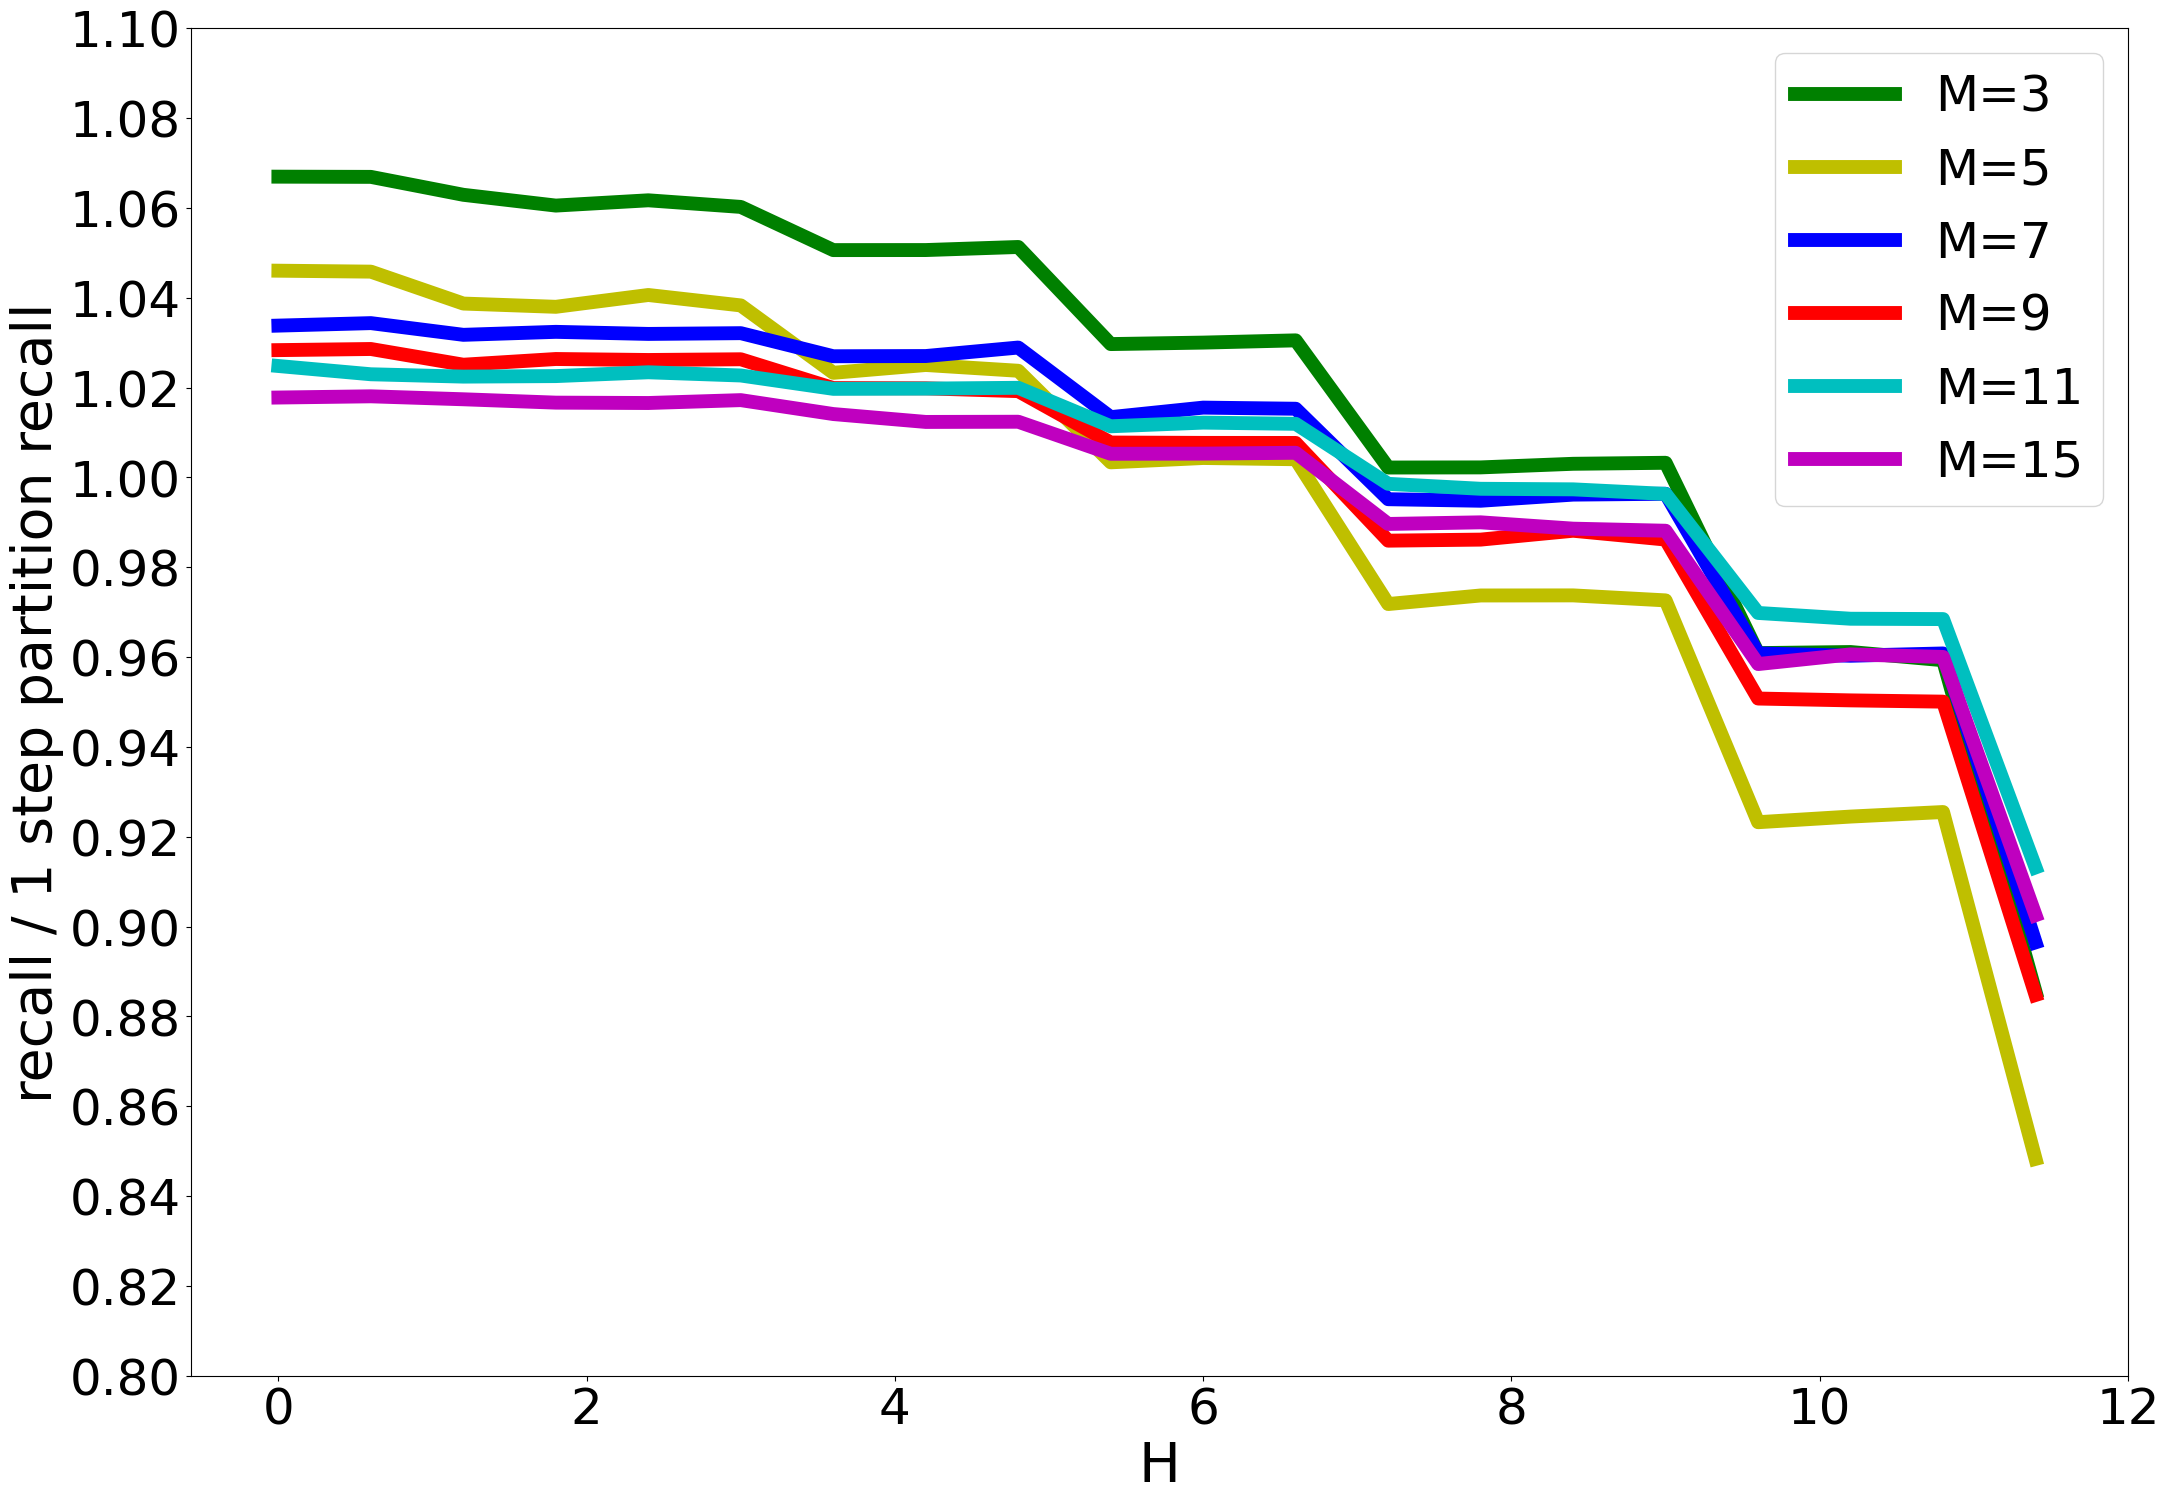
\includegraphics[width=0.7\columnwidth]{./images/First_step_win_phi_0_85_split_per_0_2_loser_0_7_m_12_new.png}
\caption{Percent of improvement of Two-Stage Partition recall over 1-step partition, for different values of $h$. All runs with $\phi = 0.85$, $k = 12$, $l = 0.7$, $f = 0.2$.}
\label{fig:First_step_win_change}
\end{figure}
For $h$ (the size of the group of candidates we pass after the first stage), we see quite the opposite picture of that of $l$. It is better for $h$ to be small, in range of $0-\frac{k}{3}$ candidates, with the precise value depending on the precise $\phi$, $k$ and $m$ (see Figure~\ref{fig:First_step_win_change}). When $k$ is larger, a higher $h$ seems to work better (as can seen in Figure~\ref{fig:size_of_high_rankk_group_for_num_of_reviews}),
perhaps because when we choose more candidates we probably will be in the top $\frac{k}{3}$ on the first round, and as number of winners decrease we need to be more cautious about those we choose. We found that higher $\phi$ values will lead to lower $h$ values,
probably since when reviewers are more noisy we also need be more cautious about the candidates we choose. When $m$ is large, a larger $h$ works better (as can seen in Figure~\ref{fig:size_of_high_rank_group_for_num_of_winners}), probably because the significant number of reviews means we have enough information about the candidate even from the first stage, allowing us to choose with confidence.

\begin{figure}[t]
\centering
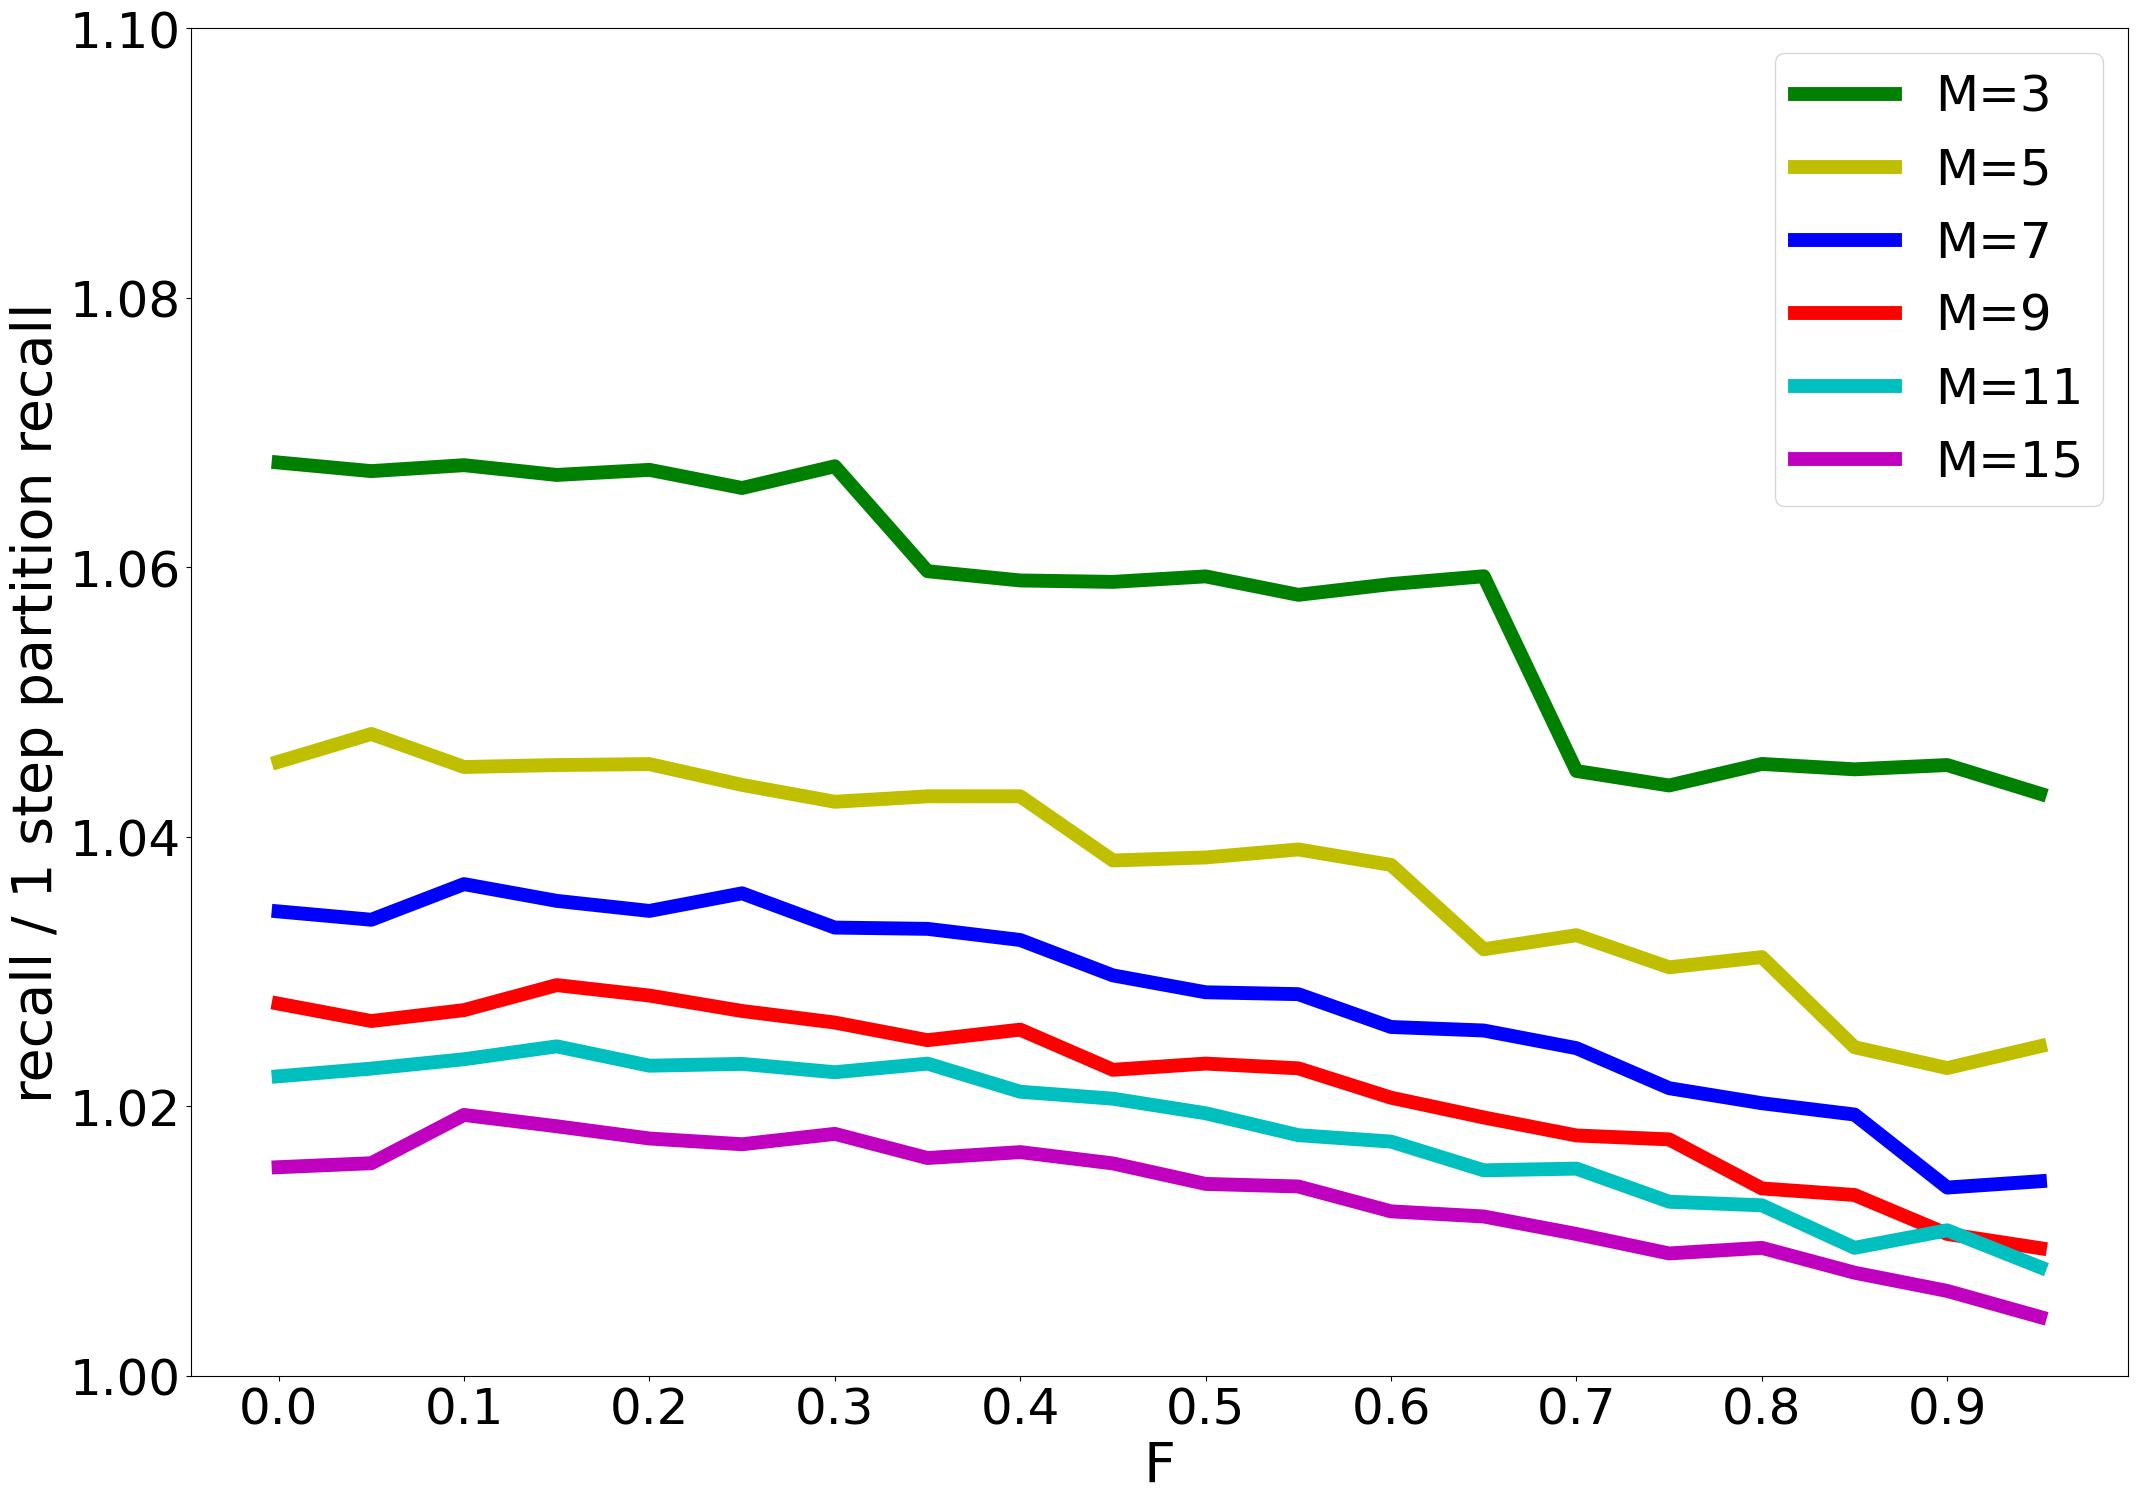
\includegraphics[width=0.7\columnwidth]{./images/split_per_phi_0_85_loser_0_7_0_2_win_group_0_m_12_new.png}
\caption{Percent of improvement of Two-Stage Partition recall over 1-step partition, for different values of $f$. All runs with $\phi = 0.85$, $k = 12$, $l = 0.7$, $h = 0$.}
\label{fig:split_per_changes}
\end{figure}


\section{Discussion}\label{disc}
In this paper we investigate using a two-stage mechanism for peer-evaluation. While the use of such mechanisms in the real-world has expanded in the past few years~\cite{LMNZCNR22}, beyond the basic intuition behind it (focusing reviews on more ``divisive'' papers), there has not been, to our knowledge, any further investigation of this idea. Here, we took the most widely explored strategyproof mechanism -- Partition -- and examined its performance when adding a Two-Stage component to it, using two different methods to implement how the mechanisms decide on which candidates to focus (a fixed set vs. a flexible, changing set of papers).

While it seems the intuition is indeed correct, and focusing on a subset of papers does improve the performance of the peer-evaluation mechanism, the improvement was not where we expected it to be. We expected the ``borderline'' papers to be more exact. That is, that the paper ranked at $k-1$ will more surely be included vs the paper ranked at $k+1$. However, our simulations showed that this is not the key benefit of the Two-Stage mechanisms, but rather the more ``middle-of-the-road'' papers. Those ranked around $\frac{k}{2}$ benefited most, as their chance of being included in the winning set increased dramatically. It seems that borderline papers are hard to differentiate, even when getting more reviews; while the better papers were able to more clearly establish their quality.

In addition we were able to explore what parameters improve the algorithms' performance best, depending on the values of $m, k,$ and $\phi$. Somewhat surprisingly, a fairly small benefit first stage suffices to help the algorithms' performance, as long as enough papers are rejected. While this may seem counter-intuitive, it seems the limited signal in the first stage is enough such that the chances of getting enough reviews to counter it is of low-enough probability to not be worth it.

There are some obvious extensions to this work: first and foremost, examining if we see similar outcomes in other peer-evaluation mechanisms. We hypothesize that we will see something similar (e.g., the two stages help the middle-of-the-road papers the most), but this has yet to be examined. Furthermore, for other mechanisms a two-stage mechanism may not be as straightforwardly strategyproof, and may require a far more complex re-working of the algorithms to accommodate a two-stage system. Beyond this, examining outcomes in distribution that are not Mallows may lead to deeper understanding of the two-stage systems (though, so far, peer-evaluation papers, requiring a ground-truth to compare themselves to, focus on Mallows distribution for comparison and quality estimates).

neque, iste reiciendis ipsum voluptas et distinctio commodi corporis sint?Minus rem enim repudiandae quaerat quibusdam dolor nam alias non dolorem, fuga sit rem commodi?Ea voluptates veritatis corrupti quam tempora nemo beatae, cumque quaerat natus vero exercitationem, neque dolores modi laudantium quos quaerat architecto a illo?Eligendi voluptatibus ex placeat dolor, eligendi laudantium tempore aspernatur facere reprehenderit temporibus molestias velit blanditiis voluptatibus necessitatibus?Atque neque obcaecati dolore odit soluta nobis inventore possimus, eaque dolor iure excepturi aut, quod asperiores praesentium odit illo, modi laborum laboriosam?Sequi dolor asperiores sapiente officia dolorum quisquam perspiciatis iusto repudiandae voluptatem deserunt, dolore culpa iste officiis itaque eaque totam nemo dolorem voluptate sapiente?Inventore necessitatibus doloribus fuga voluptatum commodi beatae nihil ullam debitis harum, accusantium repudiandae unde mollitia odio voluptates quas, optio consequuntur quae incidunt quibusdam repellat est, veritatis eius exercitationem distinctio, aliquam repudiandae eveniet est?Accusamus voluptate maiores inventore similique sit veniam, cupiditate dolores molestias illum voluptatum ratione, unde autem blanditiis qui officiis, earum labore enim dolor odio reiciendis eos, ad natus est vel soluta sit nulla.Eum provident est vero laborum vel adipisci neque explicabo ratione, facilis doloribus consequatur nesciunt ipsam tempore accusamus ducimus rem iusto nisi, molestias quisquam atque, inventore aut est dolorem voluptate dolor vitae pariatur culpa?Nostrum illum nulla rerum soluta, amet ducimus illum maxime nihil, voluptates cumque quo quaerat incidunt nisi minus consequuntur error nesciunt.Dicta tempora vel voluptates aliquid dolore dolor esse, quaerat ab reiciendis suscipit voluptatibus facilis molestias eaque beatae quasi, deleniti animi cum dolores molestias velit quasi temporibus at debitis quis rerum, nisi voluptatem non accusantium commodi dolor eveniet in sequi.Accusantium ex mollitia autem ut pariatur esse quia provident, sint perferendis repellendus ea ipsum iure nesciunt, perspiciatis dolorum molestias error possimus repellat eos at ullam, placeat aut facilis autem animi at repellendus quo dolorem sed non dolore, nemo sequi veritatis nihil quod doloribus.\clearpage
\bibliography{general}

\end{document}


